\documentclass{fiwthesis}
%\documentclass[en]{fiwthesis}   % Default language is german but can be switched to english

% ========
%  Pakete
% ========

\usepackage{textgreek}           % griechische Buchstaben außerhalb des Math-Mode
\usepackage{amsmath}             % zentrierte Formeln
\usepackage{amssymb}             % erweiterter Formelsatz mathem. Symbole

\usepackage{boldline}            % breitere Linien in Tabellen
\usepackage{booktabs}            % typographisch richtige Tabellen setzen
\usepackage{tabularx}            % Erweiterte Tabellendarstellung
\usepackage{multirow}            % Spalte über mehrere Zeilen oder Spalten ausdehnen
\usepackage{xltabular}           % Zeilenumbrüche in tabularx erlauben

\usepackage{graphicx}            % ermöglicht das Einbinden von Grafiken
\usepackage{subcaption}          % mehrere Bilder in einem Bild
\usepackage{pgfplots}            % Grafiken erzeugen
\usepackage{smartdiagram}        % schnelle und einfache Grafiken
\usepackage{pdfpages}            % Einbinden von PDFs
\usepackage{orcidlink}           % ORCID ID einbinden
\usepackage{makecell}            % Tabellenzellen formatieren
\usepackage{hologo}              % LaTeX-Logos setzen
\usepackage{svg}                 % SVG-Grafiken einbinden
\usetikzlibrary{positioning}     % bessere Ortsbezeichnung
\usetikzlibrary{shapes}          % typische Formen wie Rechtecke, Ellipsen usw. einfach zeichnen
\usetikzlibrary{intersections}   % Schnittpunkt von Geraden adressieren
\usetikzlibrary{angles, quotes}  % einfacheres Zeichnen von Winkeln
\usetikzlibrary{                 % Symbole für Schaltpläne
  circuits.logic.US,
  circuits.logic.IEC,
  circuits.logic.CDH,
  circuits.ee.IEC
}

\usepackage{lipsum}

% ===========
%  Metadaten
% ===========

\thesis{Master-Thesis}
\title{Identifikation und Vergleich von Autorenangaben zu Software zwischen verschiedenen Datenquellen}
\author{Kevin Jahrens}
\date{\today}
\matrnr{480592}
\bdate{05.08.1999}
\bcity{Bad Oldesloe}
\supervisor{\makecell[tl]{Prof.~Dr.~-Ing.~Frank Krüger\orcidlink{0000-0002-7925-3363} \\ Hochschule Wismar, Fakultät für Ingenieurwissenschaften \\ Bereich Elektrotechnik und Informatik, Wismar, Deutschland}}
\secsupervisor{\makecell[tl]{M.A.~Stephan Druskat\orcidlink{0000-0003-4925-7248} \\ Deutsches Zentrum für Luft- und Raumfahrt (DLR), \\ Institut für Softwaretechnologie, Berlin, Deutschland}}
\keywords{Data, Science, Software, Author, Comparison, Identification}

% Metadaten in die PDF-Datei schreiben
\makepdfmetadata

% ==========
%  Präambel
% ==========

% PGF Kompatibilitätseinstellung
\pgfplotsset{width=0.95\textwidth,compat=newest}

% % Bibliographie einbinden
\bibliography{quellen}

% Abkürzungen einbinden
%\gls{}         normal zu nutzen (erstes Mal: 'lange Form (kurze Form)'), danach nur 'kurze Form'
%\glspl{}       wie \gls{} nur als Plural
%\acrfull{qrc}  gibt volle Form ('lange Form (kurze Form)') egal wo
%\acrlong{qrc}  gibt lange Form ('lange Form') egal wo
%
%\newacronym{tag}{short}{long}
\newacronym{cff}{CFF}{Citation File Format}
\newacronym{pep}{PEP}{Python Enhancement Proposal}
\newacronym{pypi}{PyPI}{Python Package Index}
\newacronym{cran}{CRAN}{Comprehensive R Archive Network}
\newacronym{ner}{NER}{Named entity recognition}
\newacronym{ned}{NED}{Named entity disambiguation}
\newacronym{oss}{OSS}{Open-Source-Software}
\newacronym{doi}{DOI}{Digitaler Objektbezeichner}


% Glossar- und Abkürzungsverzeichniserstellung
\makeglossaries{}

% Index erzeugen
\makeindex[
  intoc=true,
  title=Index,
  columns=2]{}
\indexsetup{headers={\indexname}{\indexname}}

% ===============
%  Eigene Makros
% ===============

\newcommand*{\code}[1]{\texttt{#1}}

% ===============
%  Beginn Thesis
% ===============

% TODO Krüger liebt Visualisierungen davon gerne ein paar rein machen -> vllt. auch die vom Forschungsseminar übernehmen?
% TODO ich kann in der Präsentation nicht davon ausgehen, dass die Arbeit gelesen wurde! Somit muss ich auch den kompletten Kontext rüber bringen und die Ziele und was wir überhaupt machen und warum
% TODO Quellen final durch gehen (DOI benötigt keine URL und kein Zugriffsdatum)
% TODO in Quellen 6 Autoren nennen manchmal wird nur 1 genannt -> Krüger wird z. B. nicht genannt
% TODO wenn ich Simon die arbeit schicke ihm den Hinweise geben, dass mein Prof grafiken und darstellungen liebt. Er soll mich also darauf hinweisen, wo noch sowas eingebaut werden könnte/ Simon sagen, dass er die Arbeit auch gerne an seine Kollegen/ meinen künftigen Kollegen weiterleiten darf die ist eh öffentlich einsehbar wenn man weiß wo man guckt. Aber ich möchte gerne nur eine PDF mit den Kommentaren haben und nicht 20 von allen :o außerdem würde es mich freuen wenn wir die Arbeit noch etwas ausdünnen
% TODO checken, ob ich bei Zitation von software nicht nur die preferred citation zitiere sondern auch die software an sich
% TODO neue sachen immer durch languagetool jagen
% TODO nochmal alle overful boxes checken und entfernen!

\begin{document}

% ============
%  "Vorspann"
% ============

% Titelseite
\maketitle

% Aufgabenstellung
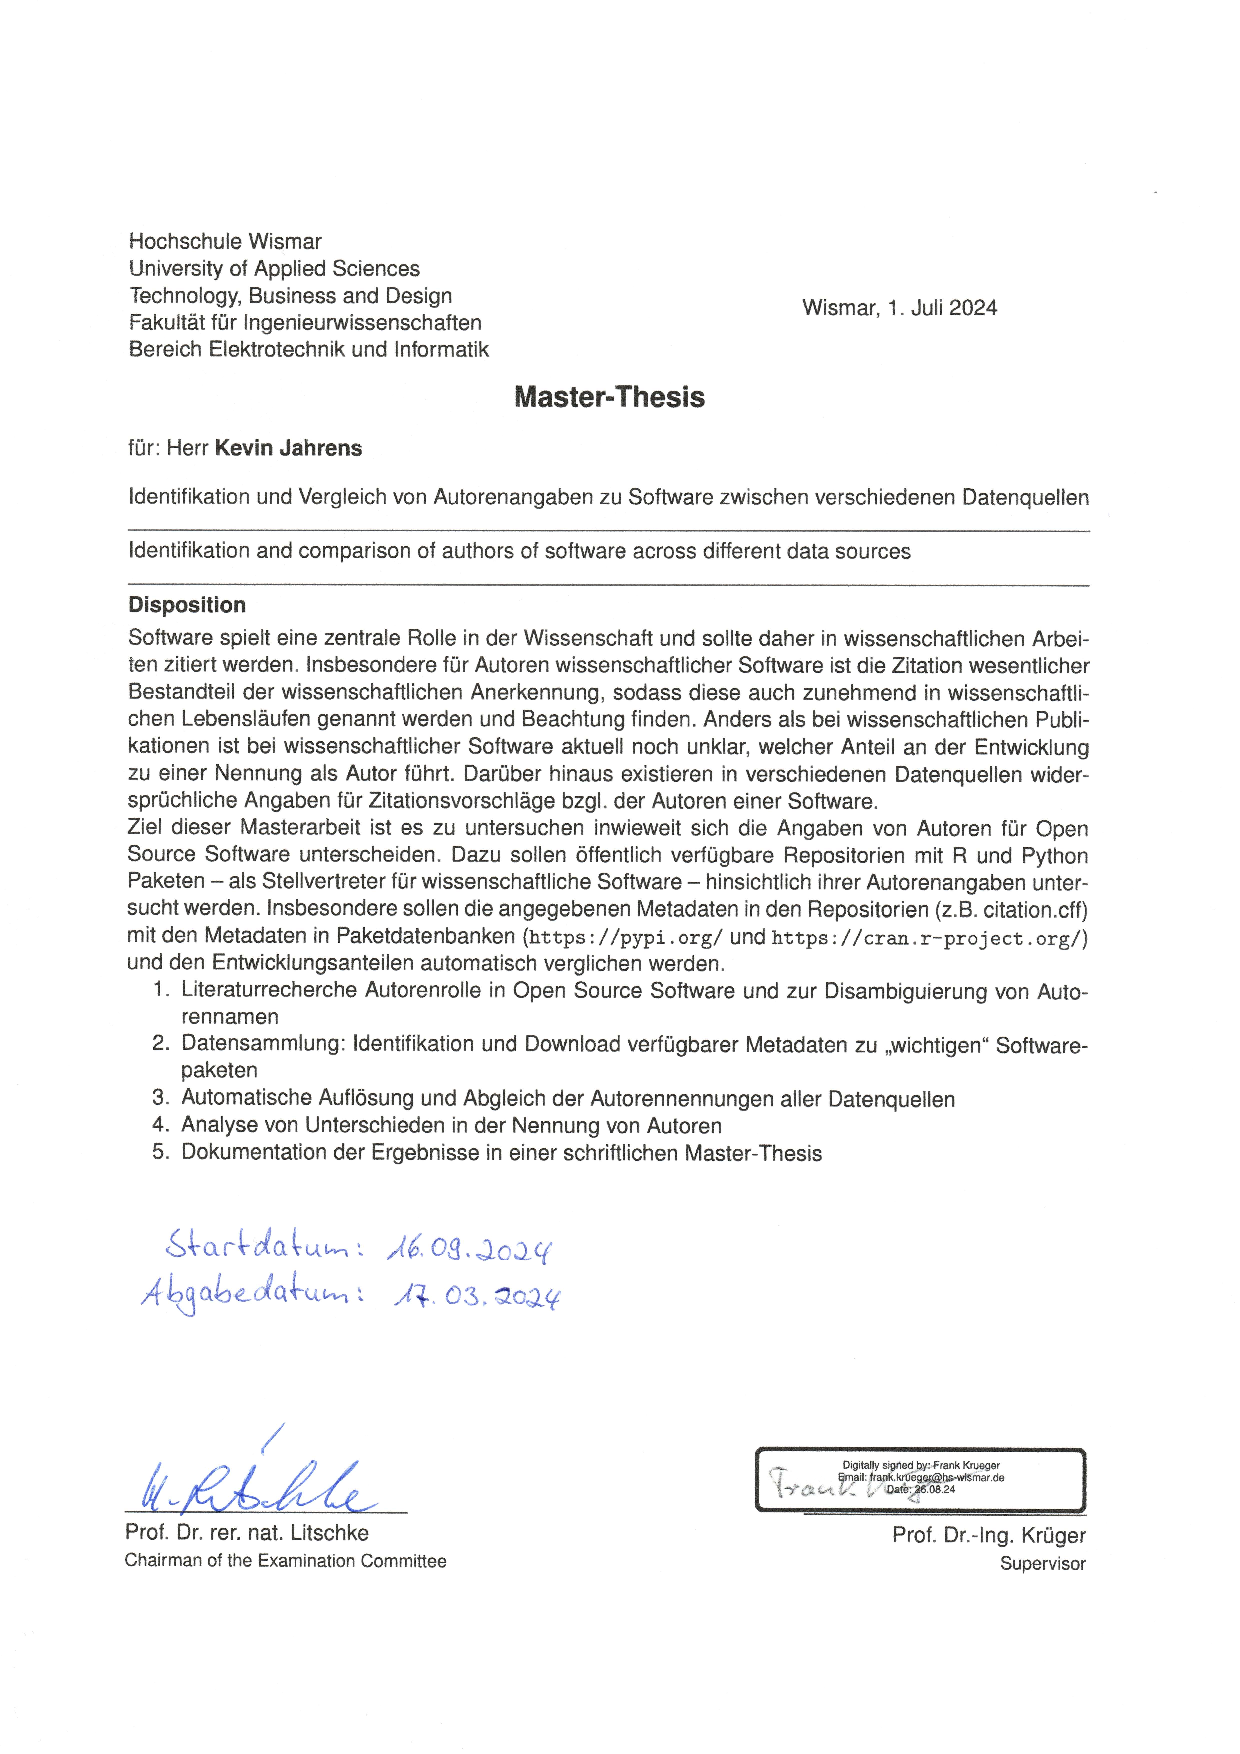
\includepdf[pages=-]{anlagen/aufgabenstellung_print.pdf}

% Abstract
\makeabstract{
  Die zunehmende Digitalisierung der Wissenschaft erhöht die Bedeutung von \gls{oss} und fordert neue Ansätze zur Anerkennung von Autoren. In dieser Arbeit werden Git-Repositorys und andere Quellen wie das \gls{cff} analysiert, um die Qualität der Autorenangaben zu ermitteln. Eine entwickelte Software extrahiert, aggregiert und visualisiert Autoreninformationen aus \gls{cran}- und \gls{pypi}-Repositorys. Die Ergebnisse zeigen Lücken bei der Nennung von Autoren in \gls{oss}. Abschließend wird anhand der Ergebnisse diskutiert, was Softwareentwickler leisten müssen, um als Autor genannt zu werden.
}{
  The increasing digitalization of science increases the importance of \acrfull{oss} and calls for new approaches to author recognition. In this work, Git repositories and other sources such as the \acrfull{cff} are analyzed to determine the quality of author information. A developed software extracts, aggregates and visualizes author information from \acrfull{cran} and \acrfull{pypi} repositories. The results show gaps in the naming of authors in \gls{oss}. Finally, the results are used to discuss what software developers need to do to be named as an author.
}

% Inhaltsverzeichnis (Schalter `compact' sorgt für einfachen Zeilenabstand)
\maketoc[compact]

% ==========
%  Textteil
% ==========

\newcolumntype{P}[1]{>{\centering\arraybackslash}p{#1}}
\newcolumntype{L}[1]{>{\raggedright\arraybackslash}p{#1}}
\newcolumntype{R}[1]{>{\raggedleft\arraybackslash}p{#1}}

\setlength{\belowcaptionskip}{\baselineskip}

% Einleitung
\chapter{Einleitung}
\label{chap:einleitung}
\section{Motivation}
\label{sec:motivation}
\section{Vorgehen}
\label{sec:vorgehen}
% TODO erklären was wird vorhaben (Autoren aus unterschiedlichen quellen extrahieren zuordnen und checken wie gut das funktioniert und wie gut Autoren von Software gepflegt werden)
\section{Gliederung}
\label{sec:gliederung}


% weitere Kapitel hier jeweils einzeln einbinden
\chapter{Grundlagen}
\label{chap:grundlagen}
% TODO ggf. TP, FN, FP, TN erklären und auch f1 score, f Score
In \autoref{sec:software-zitation} wird auf die Prinzipien der Software-Zitation eingegangen.
Es wird beschrieben, warum die Zitation von Software ebenfalls wichtig ist, ähnlich wie die Zitation von anderen wissenschaftlichen Arbeiten.
Außerdem wird darauf eingegangen, dass ebenfalls Personen zitiert werden sollten, welche nicht aktiv an der Software programmieren.
Zusätzlich dazu wird in \autoref{sec:autorenrolle-oss} auf die Rolle von Autoren in \gls{oss} eingegangen und ein wissenschaftliches Paper dargestellt, welches dies schon analysiert hat.

Autoren von Software werden in unterschiedlichen Quellen zitiert.
Einige dieser Quellen sind stark mit der Softwareentwicklung verbunden.
So gibt es verschiedene Systeme, die ein Entwickler verwenden kann, um seine Arbeit zu erleichtern bzw. überhaupt sinnvoll zu ermöglichen, in denen Sie anschließend als Autoren genannt werden.
In den Abschnitten \ref{sec:versionsverwaltung} und \ref{sec:paketverwaltung} wird auf die Versions- und Paketverwaltung eingegangen, welche zwei dieser Systeme darstellen.
Des Weiteren existieren spezielle Zitierformate, in welchen Autoren explizit angegeben werden können.
Auf diese Formate wird in \autoref{sec:zitierformate} eingegangen.
Außerdem können in Fließtexten, beispielsweise der Beschreibung einer Software, ebenfalls Autoren genannt werden.
In \autoref{sec:named-entity-recognition} wird auf die \emph{Named Entity Recognition} eingegangen, welche eine Methode darstellt, um Personen in Texten zu erkennen.

Alle Quellen, welche beschrieben werden, dienen im Verlauf der Masterarbeit als Grundlage für die Extraktion von Autoren und deren Metainformationen.
Die extrahierten Autoren müssen anschließend zugeordnet werden.
Der Prozess dafür heißt \emph{Author Name Disambiguation}, welcher in \autoref{sec:author-name-disambiguation} beschrieben wird.
Eine weitere einfache Möglichkeit des Abgleichs ist ein einfacher Abgleich von Zeichenfolgen.
Dieser funktioniert jedoch nicht immer, da Autoren unterschiedliche Schreibweisen ihres Namens verwenden können.
Aus diesem Grund wird in \autoref{sec:unscharfe-suche} auf die unscharfe Suche eingegangen, welche eine Möglichkeit darstellt, um ähnliche Zeichenfolgen miteinander zu vergleichen, beispielsweise für den Abgleich von Namen mit oder ohne genannten Zwischennamen.
\section{Zitation von Software}
\label{sec:software-zitation}
Software ist ein wesentlicher Bestandteil moderner Forschung.
In der wissenschaftlichen Literatur ist es üblich, Quellen zu zitieren, um die Nachvollziehbarkeit und Reproduzierbarkeit von wissenschaftlichen Arbeiten zu gewährleisten.
Im Gegensatz dazu ist dies bei wissenschaftlicher Software aktuell in diesem Umfang noch nicht gegeben.
Hier gibt es aktuell kaum Anerkennung und Unterstützung für die Leistungen einzelner Autoren.
Aus diesem Grund hat die \glqq FORCE11 Software Zitier Arbeitsgruppe\grqq{} Prinzipien der Software Zitation erstellt, welche eine breite Akzeptanz in der wissenschaftlichen Gemeinschaft finden sollen.
Im Folgenden werden die Prinzipien vorgestellt und erläutert \cite{smith_software_2016}:

\begin{enumerate}
    \item \textbf{Wichtigkeit:} Software sollte ein seriöses und zitierbares Produkt wissenschaftlicher Arbeit sein. Software Zitierungen sollten im wissenschaftlichen Kontext die gleiche Bedeutung zugeschrieben bekommen wie Zitierungen anderer Forschungsprodukte, wie Publikationen. Sie sollten wie Publikationen auch in der Arbeit enthalten sein, zum Beispiel in der Referenzliste eines Artikels. Software sollte auf derselben Grundlage zitiert werden wie jedes andere Forschungsprodukt auch, wie zum Beispiel ein Aufsatz oder ein Buch. Das bedeutet, dass Autoren die entsprechend verwendete Software zitieren sollten, so wie sie die entsprechenden Publikationen zitieren würden.
    \item \textbf{Anerkennung und Zuschreibung:} Softwarezitate sollten die wissenschaftliche Anerkennung und die normative, rechtliche Würdigung aller Mitwirkenden an der Software ermöglichen, wobei anerkannt wird, dass ein einziger Stil oder ein Mechanismus für die Namensnennung nicht auf jede Software anwendbar sein kann.
    \item \textbf{Eindeutige Identifikation:} Ein Softwarezitat sollte eine Methode zur Identifikation enthalten, die maschinell verwertbar, weltweit eindeutig und interoperabel ist und zumindest von einer Gemeinschaft der entsprechenden Fachleute und vorzugsweise von allgemeinen Forschern anerkannt wird.
    \item \textbf{Persistenz:} Eindeutige Identifikatoren und Metadaten, die die Software und ihre Verwendung beschreiben, sollten bestehen bleiben – auch über die Lebensdauer der Software hinaus, die sie beschreiben.
    \item \textbf{Zugänglichkeit:} Softwarezitate sollten den Zugang zur Software selbst und zu den zugehörigen Metadaten, Dokumentationen, Daten und anderen Materialien erleichtern, die sowohl für Menschen als auch für Maschinen notwendig sind, um die referenzierte Software sachkundig nutzen zu können.
    \item \textbf{Spezifizität:} Softwarezitate sollten die Identifizierung und den Zugang zu der spezifischen Version der verwendeten Software erleichtern. Die Identifizierung der Software sollte so spezifisch wie nötig sein, z. B. durch Versionsnummern, Revisionsnummern oder Varianten wie Plattformen.
\end{enumerate}

In dieser Arbeit wird verstärkt auf das Prinzip der Wichtigkeit eingegangen, da besonders im \gls{cff} und Bib\TeX{} Format die Möglichkeit besteht nicht die Software, sondern beispielsweise ein Artikel anzugeben.
Diese Zitierweise würde dann das Prinzip der Wichtigkeit verletzen, da die Software nicht die gleiche Bedeutung zugeschrieben bekommt wie andere Forschungsprodukte.
Diese Diskrepanz wird in \autoref{chap:ergebnisse} dargestellt.

Es gibt verschiedene Gründe, warum die Zitation von Software ebenfalls wichtig ist und auch, dass Standards der Zitation eingehalten werden, ähnlich wie es der Fall bei anderen wissenschaftlichen Arbeiten ist.
Einige dieser Gründe werden im Folgenden genannt \autocite{smith_software_2016}:

\begin{itemize}
    \item Forschungsfelder verstehen: Software ist ein Produkt der Forschung und wenn sie nicht zitiert wird, werden Lücken in der Aufzeichnung der Forschung über den Fortschritt in diesem Forschungsfeld entstehen.
    \item Anerkennung: Akademische Forscher auf allen Ebenen, einschließlich Studenten, Postdocs, Dozenten und Mitarbeiter, sollten für die Softwareprodukte, die sie entwickeln und zu denen sie beitragen, anerkannt werden, insbesondere wenn diese Produkte die Forschung anderer ermöglichen oder fördern. Nicht-akademische Forscher sollten ebenfalls für ihre Softwarearbeit anerkannt werden, obwohl die spezifischen Formen der Anerkennung sich von denen für akademische Forscher unterscheiden.
    \item Software entdecken: Mithilfe von Zitaten kann die in einem Forschungsprodukt verwendete Software gefunden werden. Weitere Forscher können dann dieselbe Software für andere Zwecke verwenden, was zu einer Anerkennung der für die Software Verantwortlichen führt.
    \item Reproduzierbarkeit: Die Angabe der verwendeten Software ist für die Reproduzierbarkeit notwendig, aber nicht ausreichend. Zusätzliche Informationen wie Konfigurationen und Probleme auf der Plattform sind ebenfalls erforderlich.
\end{itemize}

Wie bereits erwähnt werden Autoren in unterschiedlichen Quellen angegeben.
Einige dieser Quellen werden in dieser Masterarbeit untersucht, wie beispielsweise das \gls{cff} und Bib\TeX{} Format.
Die Autoren in diesen Quellen werden von dem jeweiligen Softwareprojekt angegeben.
Falls an dem Projekt nicht nur Softwareentwickler beteiligt sind, sondern beispielsweise auch Grafikdesigner oder Übersetzer, so sollten diese ebenfalls in den Quellen angegeben werden.
Dies ist wichtig, da diese Personen ebenfalls einen Beitrag zum Projekt geleistet haben und somit auch Anerkennung verdienen.

Es gibt ebenfalls bereits Projekte, welche sich für die halb automatische Nennung von Autoren ohne Code Beitrag einsetzen.
Ein Beispiel für ein solches Projekt ist \glqq All Contributors\grqq{} \autocite{all_contributors_recognize_2024}.
Bei der Verwendung von \glqq All Contributors\grqq{} werden die Mitwirkenden jedoch nicht in einem speziellen Format angegeben, sondern standardmäßig in der README-Datei, welche im Projekt enthalten ist.
Die Liste wird dabei von einem Bot automatisch generiert und aktualisiert, sodass sie der Spezifikation von \glqq All Contributors\grqq{} entspricht.
Über einen Befehl in einem Issue oder einem Pull Request kann ein neuer Mitwirkender hinzugefügt werden.
Autoren, welche keinen Code beigetragen haben, stellen im weiteren Verlauf der Masterarbeit ein Problem dar, da diese nicht mit den Autoren aus den Quellen abgeglichen werden können, da sie keine Commits haben.
Dies wird in \autoref{sec:abgleich} genauer erläutert.

% TODO darauf noch eingehen? https://google.github.io/opencasebook/authorship/
Die untersuchten Pakete in dieser Arbeit sind Open Source, welche auf GitHub veröffentlicht werden.
Open Source Software ist Software, deren Quellcode öffentlich zugänglich ist und von einer Gemeinschaft von Entwicklern entwickelt wird.
Die Entwickler arbeiten dabei in der Regel ehrenamtlich und ohne Bezahlung an der Software, wobei einige der untersuchten Pakete auch von Organisationen veröffentlicht werden, wie beispielsweise die \glqq google-auth-library-python
\grqq{} von Google.
Diese wird primär von Google Mitarbeitern entwickelt und gepflegt.
Wie bereits beschrieben sind Prinzipien und Gründe definiert, warum Software ebenfalls zitiert werden sollte.
Welche Autoren in den Quellen angegeben werden sollten, ist jedoch nicht so genau definiert wie es beispielsweise im Bereich von wissenschaftlichen medizinischen Artikel der Fall ist.
In diesem Bereich hat das \glqq International Commitee of Medical Journal Editors\grqq{} Richtlinien für die Rolle von Autoren und Beitragenden in wissenschaftlichen Artikeln definiert \autocite{noauthor_icmje_nodate}.
Unter anderem aus diesem Grund ist die Menge der Autoren, welche in den Quellen angegeben werden, unterschiedlich und hängt von dem jeweiligen Projekt ab.
Außerdem ist es möglich, dass ausschließlich Autoren in den Quellen angegeben werden, welche aktuell nicht mehr an dem Projekt beteiligt sind, aber beispielsweise vor fünf Jahren aktiv das Projekt geführt haben.
Diese und weitere Auffälligkeiten werden in der Masterarbeit untersucht.
Auch dies ist in anderen Bereichen anders definiert, sodass auch die neuen Autoren genannt werden müssen wie beispielsweise bei Neuauflagen von Büchern.

\section{Autorenrolle und Anerkennung in Open-Source-Software}
\label{sec:autorenrolle-oss}
% TODO ggf. noch mehr schreiben?
% TODO ggf. weitere Paper?
In der Wissenschaft existieren bereits Analysen zur Rolle von Autoren in \gls{oss}.
Ein Paper analysiert die Zuschreibung von Entwicklern in \gls{oss} \autocite{young_which_2021}.
Sie beantworten in dem Paper folgende Fragen:

\begin{itemize}
  \item Wie unterscheiden sich die Modelle für die Anerkennung von Beiträgen?
  \item Wie viele Informationen gehen verloren, bei einer Festlegung auf Repository-Änderungen als Modell für den Beitrag?
  \item Wie entwickeln sich die Beiträge zu \gls{oss} über die Zeit?
  \item Können wir Projekte auf der Grundlage von Beitragsmustern klassifizieren?
\end{itemize}

In dem Paper werden vier Modelle für die Anerkennung unterschieden.
Im ersten Modell werden die Änderungen an einem Repository als Beitrag betrachtet.
Dabei wird auf die Top 100 Benutzer in den Projekten geschaut, wie sie durch die GitHub API ausgegeben werden.
Das zweite Modell betrachtet die Autoren, welche automatisch über ein Tool identifiziert werden.
In dem Paper wird hierbei das Programm \textit{octohatrack} verwendet \autocites{young_which_2021}{noauthor_labhroctohatrack_2024}.
Als drittes Modell werden die Autoren mittels Taxonomien identifiziert.
Hierbei wird die \mintinline{text}{.all-contributorsrc}-Datei von \glqq All Contributors\grqq{} analysiert \autocites{young_which_2021}{all_contributors_recognize_2024}.
Das vierte Modell betrachtet die Autoren, welche mittels ad hoc Methoden identifiziert werden.
Diese können beispielsweise durch die Analyse von nicht standardisierten Quellen stammen wie beispielsweise Webseiten oder unstrukturierten Textdateien.
Das Modell wird in dem Paper aufgrund der Komplexität nicht fokussiert betrachtet.

Die Autoren betrachten die Fragen und Modelle dabei von einer gehobenen Perspektive.
Dabei werden die einzelnen Fragen mithilfe von verschiedenen generellen Metriken wie die Anzahl der Autoren, welche Commits erstellt haben oder als Autoren in \glqq All Contributors\grqq{} genannt werden, beantwortet.
Sie betrachten keine einzelnen Autoren oder Projekte, sondern analysieren die gesamte \gls{oss}-Landschaft primär auf Basis von der Anzahl der Autoren.
Es werden keine genaueren Analysen durchgeführt wie beispielsweise in dieser Masterarbeit, in der unter anderem betrachtet wird, ob die genannten Autoren noch aktiv an dem Projekt beteiligt sind.
Außerdem wird nicht auf Daten eingegangen, welche aus weiteren Quellen wie dem \gls{cff} oder \hologo{BibTeX} Format stammen.

\section{Versionsverwaltung}
\label{sec:versionsverwaltung}
% TODO Das ändern ist erstmal nur kopiert und auch anpassen wie zitiert wird er mag es nicht wenn ganze abschnitte eine quelle haben. Immer nur den Teil der wirklich aus der Quelle ist zitieren
% TODO noch mehr schreiben sollte auf 3 Seiten kommen
% TODO Issue und Pull Request in der Versionsverwaltung erwähnen und erklären
% TODO auf Github eingehen was das ist und wofür das benutzt wird
Die Versionsverwaltung ist ein System, um verschiedene Versionen von Software zu verwalten.
Es bietet Zugang zu Code und dessen Änderungen in der Vergangenheit.
Der Code und getätigte Änderungen werden in einem Repository gespeichert.
Dadurch ist die Versionsverwaltung eine Art Logbuch, in dem alle Änderungen festgehalten werden.
Dabei wird zusätzlich zu der Änderung der Autor und der Zeitpunkt der Änderung festgehalten.
Dies ermöglicht es in dem Forschungsseminar empirisch die Menge an Arbeit der einzelnen Autoren zu ermitteln. \autocite{ponuthorai_version_2022}

Es gibt zwei verschiedene Arten von Versionsverwaltungssystemen.
Zum einen gibt es die zentralen Systeme, bei denen alle Änderungen zentral verwaltet werden, beispielsweise SVN.
Zum anderen gibt es die verteilten Systeme, bei denen jeder Entwickler eine Kopie des gesamten Repository und dessen Vergangenheit hat.
Ein solches System ist Git, welches sich mit einem Marktanteil von ungefähr 75 \% gegenüber anderen Systemen durchgesetzt hat \autocite{lindner_version_2024}.
Aus diesem Grund und weil Git-Repositorys in der Arbeit untersucht werden, wird auf Git eingegangen.
Dabei werden Begriffe erklärt, mit denen es möglich ist, die geleistete Arbeit von einzelnen Autoren innerhalb eines Repositorys zu untersuchen. \autocite{ponuthorai_version_2022}

In Repositorys gibt es verschiedene Arten von Statistiken.
In Git werden Revisionen als ein \emph{Snapshot} gespeichert.
Anders als in anderen Systemen wird keine Serie von Änderungen gespeichert, sondern ein \emph{Snapshot} der Änderungen zu einem bestimmten Zeitpunkt erstellt.
Dies wird ein Commit genannt.
An einem Commit werden verschiedene Metainformationen gespeichert.
Unter anderem wird eine Commit-Nachricht, der Autor und der Zeitpunkt der Änderungen gespeichert.
Mehrere Commits bilden die Commit-Historie bzw. die Vergangenheit eines Repositorys.
Weitere Eigenschaften, welche sich aus dem Repository exportieren lassen, sind die Anzahl der eingefügten und gelöschten Zeilen.
Außerdem lässt sich die Anzahl der geänderten Dateien ermitteln.
Diese Werte können für das gesamte Repository oder für einzelne Autoren ermittelt werden. \autocite{ponuthorai_version_2022}

Die Statistiken der Repositorys können auf verschiedene Arten aufgearbeitet werden.
Zum einen können einige direkt mittels Git-Befehlen ausgelesen werden \autocite{chacon_git_2024}.
Andere wiederum benötigen komplexere Abfragen, welche beispielsweise mittels Skripten oder speziellen Programmen ausgelesen werden können.
Ein Beispiel für ein Programm, welches Git-Statistiken aufarbeitet, ist \emph{git-quick-stats} \autocite{mestan_git-quick-stats_2024}.
Außerdem bieten Onlinedienste zur Versionsverwaltung, wie GitHub, Statistiken über APIs an, welche jedoch im Umfang der Anfragen limitiert sind \autocite{github_rate_2022}.

\section{Software-Verzeichnisse und Paketverwaltung}
\label{sec:paketverwaltung}
Im Gegensatz zur Versionsverwaltung verwaltet die Paketverwaltung keinen Code und dessen Änderungen, sondern fertige Softwarepakete, welche von Entwicklern erstellt und in einem Software-Verzeichnis abgelegt werden.
Inhalt eines Pakets können beispielsweise standardisierter Code von Software-Modulen sein oder kompilierter Code.
Zusätzlich werden in einem Paket Metadaten gespeichert.
Diese Metadaten können beispielsweise eine Beschreibung, Version, Abhängigkeiten und Autoren des Pakets enthalten.
Sie lassen sich aus dem Paket mithilfe des Paketverwaltungssystems auslesen oder über APIs des Software-Verzeichnisses abrufen.
Außerdem übernimmt das Paketverwaltungssystem das Installieren und meistens auch das Aktualisieren und Deinstallieren von Paketen.
Zusätzlich wird das System verwendet, um fehlende Abhängigkeiten von Paketen automatisch zu installieren \autocite{spinellis_package_2012}.

In dieser Arbeit wird auf zwei Software-Verzeichnisse eingegangen.
Zum einen wird auf \gls{pypi} eingegangen, welches das Verzeichnis für Python ist und von der Paketverwaltung \emph{pip} verwendet wird.
Zum anderen wird auf \gls{cran} eingegangen, welches das Verzeichnis für R ist.
In \gls{pypi} sind aktuell mehr als 500.000 unterschiedliche Projekte mit über 5 Millionen Veröffentlichungen verfügbar \autocite{python_software_foundation_pypi_2024}.
Im Gegensatz dazu sind in \gls{cran} aktuell mehr als 20.000 Pakete verfügbar \autocite{cran_team_comprehensive_2024}.

\subsection{PyPI}
\label{subsec:paketverwaltung_pypi}
\gls{pypi} hat zu Beginn des Jahres 2024 ein \gls{pep} veröffentlicht, welches die Verifizierung von Daten auf \gls{pypi} beschreibt \autocite{python_software_foundation_pep_2024}.
In dem \gls{pep} werden Änderungen an der API beschrieben, welche zum Hochladen von Paketen genutzt wird, um sogenannte \glqq Attestation objects\grqq{} zu unterstützen, in denen digitale Signaturen enthalten sind.
Das Ziel ist es verifizierte Daten auf \gls{pypi} zu ermöglichen, sodass Anwender direkt erkennen können, ob die Daten vertrauenswürdig sind.
Aktuell wird dieses \gls{pep} umgesetzt, wodurch es zu vielen Änderungen in der API und auch in der Weboberfläche von \gls{pypi} kommt.

Außerdem sind noch nicht alle Daten über die APIs erreichbar und es ist auch aktuell nicht über die API erkennbar, ob es sich um verifizierte oder nicht verifizierte Daten handelt.
Ein Beispiel für verifizierte Daten sind Links, beispielsweise zu GitHub.
Diese Links werden von \gls{pypi} als verifiziert angesehen, wenn der Upload des Pakets auf \gls{pypi} über eine GitHub-Action erfolgt.
Zudem werden die Personen als verifiziert dargestellt, welche in \gls{pypi} als Owner oder Betreuer des Pakets eingetragen sind, sie haben somit einen Account bei \gls{pypi}.
Der dargestellte Owner kann nicht über eine API abgefragt werden.

Die dargestellten GitHub-Statistiken werden dabei von \gls{pypi} ermittelt und nicht über APIs ausgegeben.
Das Ziel von \gls{pypi} ist es, dass alle Daten verifiziert werden können und keine Daten in der unverifizierten Form vorliegen.

\begin{figure}
    \begin{center}
        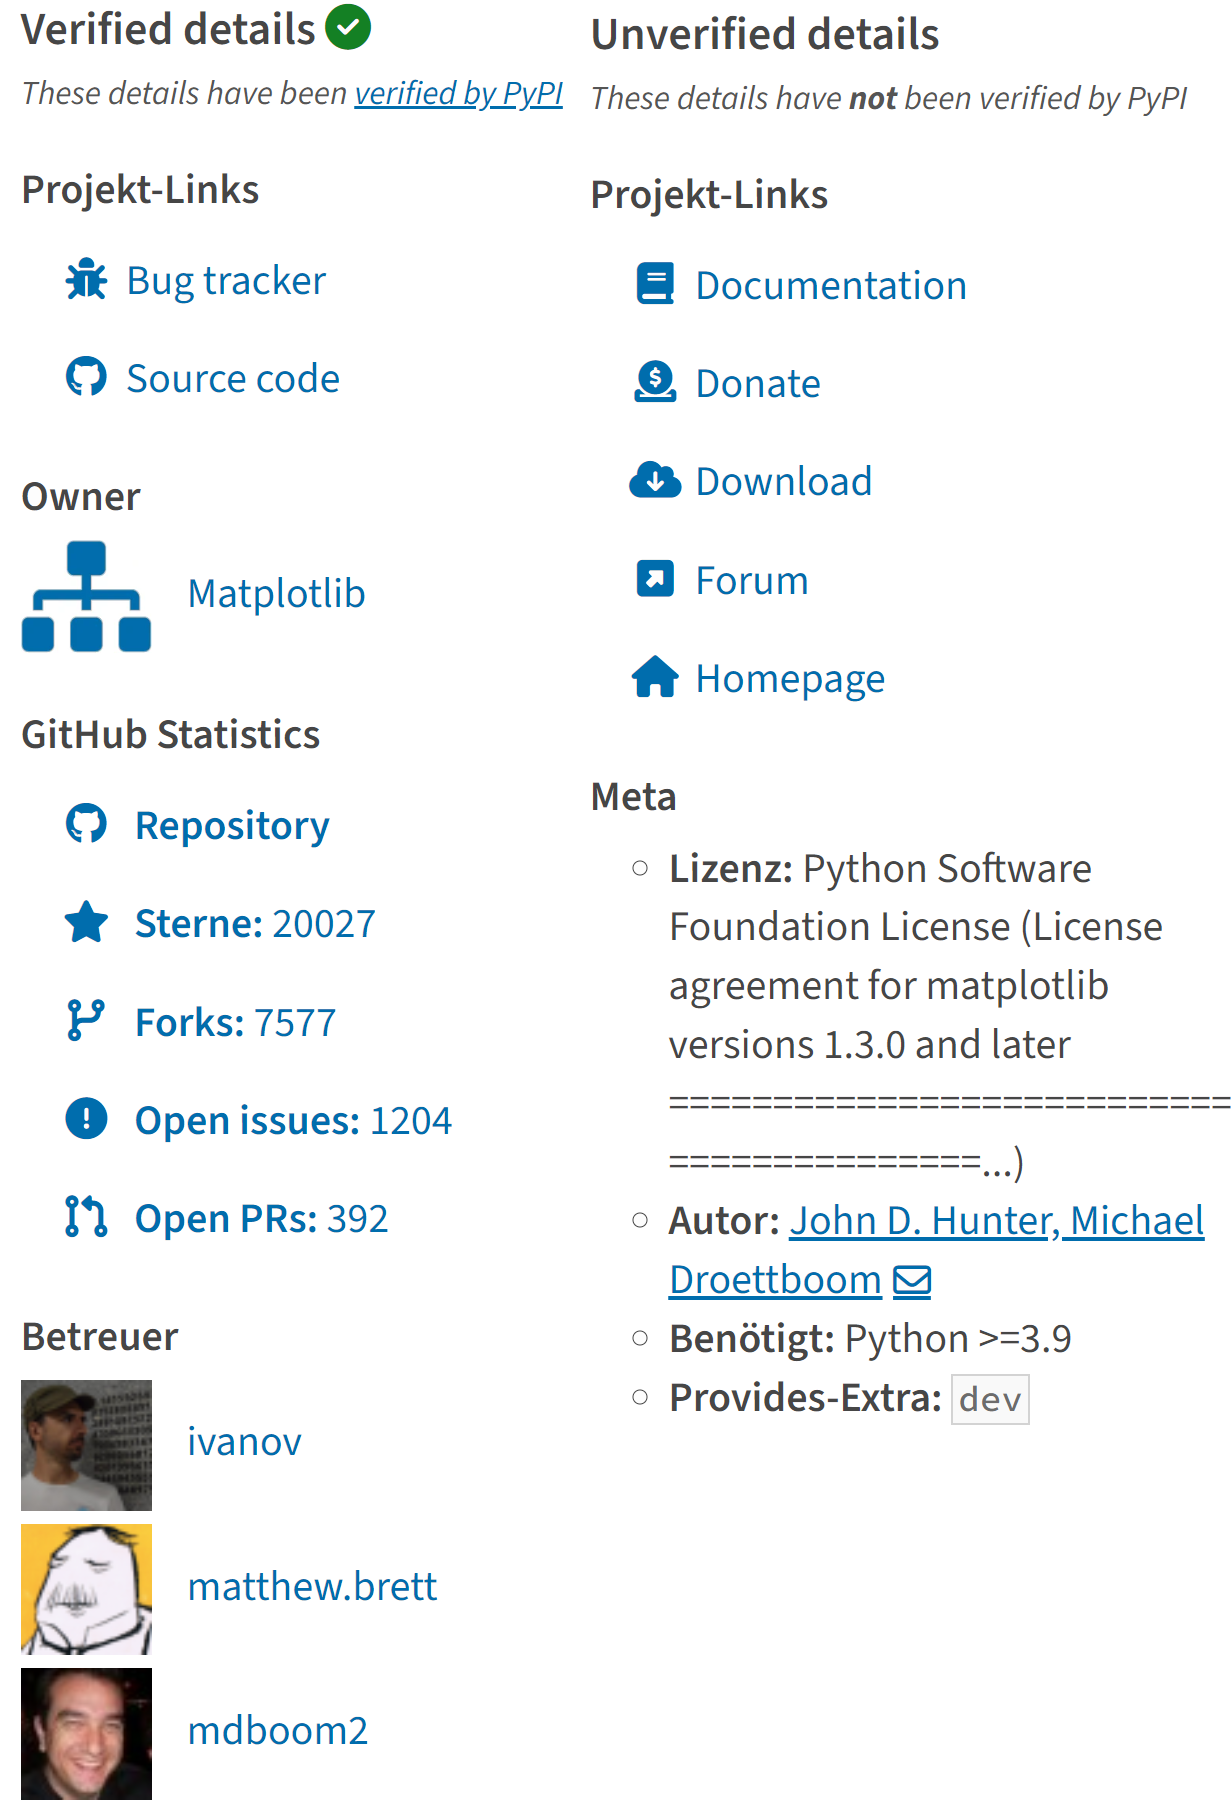
\includegraphics[width=0.95\textwidth]{bilder/pypi.png}
    \end{center}
    \caption{\gls{pypi} Verifizierte und unverifizierte Daten}
    \label{fig:pypi_verified_unverified_details}
    \small
    Die Abbildung stellt die verifizierten und unverifizierten Daten des Pakets \emph{matplotlib} auf \gls{pypi} dar \autocite{python_software_foundation_pypi_2024}.
\end{figure}

\gls{pypi} bietet verschiedene APIs und Quellen an, um die Daten der Pakete abzufragen.
Im Folgenden werden auf einige der Zugriffsmöglichkeiten eingegangen, welche mit Ausnahme der BigQuery alle in dieser Arbeit verwendet werden.

\subsubsection*{JSON-API}
\label{subsubsec:pypi_json_api}
% TODO ggf. die nicht verifizierten Daten stammen aus der Python toml (stammen die Daten wirklich alle aus der toml?) Falls ja das erwähnen und erklären, dass die Daten direkt von dem Python-Paket stammen und pypi diese nur durchreicht
Die JSON-API ist die bevorzugt zu verwendende API von \gls{pypi} und bietet die Möglichkeit, die Metadaten eines Pakets abzufragen \autocite{python_software_foundation_warehouse_2024}.
Diese API ist nicht in der Anzahl der Anfragen beschränkt.
Daten der neuesten Version des Pakets werden von der API zurückgegeben.
Die Werte in den Metadaten stammen aus den Daten, welche beim Hochladen auf \gls{pypi} angegeben wurden.
Die Daten des ersten Uploads eines Releases werden dabei als Metadaten der Version gespeichert und bei weiteren Uploads dieser Version nicht überschrieben.

Inhalt der Metadaten sind beispielsweise die Autoren und Maintainer zuzüglich deren E-Mail-Adresse, die Beschreibung, Lizenz und Links zu unterschiedlichen Quellen, beispielsweise einem GitHub-Repository \autocite{python_software_foundation_warehouse_2024}.
Die Beschreibung kann den Text aus der README-Datei des Pakets auf GitHub enthalten.
Es ist jedoch auch möglich, eine eigene Beschreibung für \gls{pypi} anzugeben, sodass sich die README-Datei in GitHub und die Beschreibung auf \gls{pypi} unterscheiden können.
Die Metadaten werden von den Entwicklern des Pakets eingetragen.
In \autoref{fig:pypi_verified_unverified_details} sind einige der Metadaten des Pakets \emph{matplotlib} unter dem Punkt \glqq Meta\grqq{} dargestellt.
Weitere Daten sind unter dem Punkt \glqq Projekt-Links\grqq{} unter den verifizierten Details dargestellt.

Die Autoren und Maintainer aus den Metadaten müssen nicht den verifizierten Betreuern und Owner des Pakets auf \gls{pypi} entsprechen, da dies unterschiedliche Systeme sind.
Zum einen sind es die Benutzer, welche Rechte auf \gls{pypi} haben, um das Paket dort anzupassen und zum anderen sind es die Personen, welche durch die Entwickler des Pakets angegeben werden.
Die Autoren und Maintainer können jedoch ebenfalls verifiziert sein, wobei dies über die API noch nicht abgefragt werden kann, jedoch in der Weboberfläche bereits für einige Pakete dargestellt wird.
Es gibt aktuell wenig Pakete, bei denen die Autoren verifiziert sind, ein Beispiel ist das Paket \emph{hololinked}, welches zum Zeitpunkt des Schreibens darüber verfügt.
\emph{Matplotlib} unterstützt dies aktuell noch nicht, wie in \autoref{fig:pypi_verified_unverified_details} dargestellt ist.
Die verifizierten Betreuer und Owner können aktuell nicht über die JSON-API abgefragt werden, sondern müssen über die XML-RPC-API abgefragt werden, da diese die einzige API ist, welche die Daten zur Verfügung stellt.

\subsubsection*{PyPI XML-RPC}
\label{subsubsec:pypi_xml_rpc}
Die \gls{pypi} XML-RPC-API ist eine veraltete API, welche jedoch noch genutzt werden kann, um einige Informationen zu den Paketen abzufragen.
Es wird empfohlen, diese API nicht mehr zu verwenden und auf den RSS-Feed oder die JSON-API umzusteigen \autocite{python_software_foundation_warehouse_2024}.
Dadurch ist die API in der Anzahl der möglichen Anfragen stark limitiert und auch die Abstände zwischen den Anfragen müssen relativ groß sein.
\gls{pypi} macht keine genauen Angaben darüber, wie viele Anfragen in welchem Zeitraum möglich sind.
Diese API ist jedoch die einzige Quelle, um die Betreuer eines Pakets abzufragen, ohne einen Web-Scraper einsetzen zu müssen.
Web-Scraping bezeichnet dabei das Extrahieren von Daten aus Webseiten, indem der HTML-Code der Webseite analysiert wird \autocite{richardson_beautifulsoup4_2024}.

Die Betreuer, welche über die API ausgegeben werden, enthalten den Benutzernamen auf \gls{pypi}, ein Vollname wird hierbei nicht ausgegeben.
Außerdem enthalten sie eine Rollenbezeichnung, welche entweder \emph{Maintainer} oder \emph{Owner} sein kann, welcher in der Oberfläche nicht dargestellt wird.
Owner können dabei alle Änderungen am \gls{pypi} Projekt vornehmen und Betreuer können neue Versionen des Pakets veröffentlichen \autocite{ingram_deprecate_2023}.
Der Benutzername für die Betreuer des Pakets \emph{matplotlib} sind in \autoref{fig:pypi_verified_unverified_details} unter dem Punkt \glqq Betreuer\grqq{} dargestellt.
Aktuell stellt \gls{pypi} keine API bereit, um den Namen eines Benutzers abzufragen, sodass nur der Benutzername über eine API abgefragt werden kann \autocite{python_software_foundation_add_2024}.

\subsubsection*{BigQuery}
\label{subsubsec:pypi_bigquery}
Ebenfalls bietet \gls{pypi} über Google BigQuery einen Datensatz an, in dem alle Pakete mit ihren Versionen und Metadaten enthalten sind \autocite{python_software_foundation_warehouse_2024}.
BigQuery ist ein Dienst von Google, welcher auf der Infrastruktur der Google Cloud-Plattform ausgeführt wird \autocite{google_bigquery_2024}.
Es ist möglich, den kompletten Datensatz auf BigQuery in mehreren einzelnen CSV-Dateien herunterzuladen.
Dabei kann ausgewählt werden, welche Daten heruntergeladen werden sollen.

Nicht alle Metadaten, welche über die JSON-API abgefragt werden können, stehen in der BigQuery zur Verfügung.
Ebenfalls stehen nicht alle Daten der BigQuery in der JSON-API zur Verfügung.
Die wichtigsten Daten sind in beiden Quellen enthalten.
So sind beispielsweise der Autor und Maintainer und deren E-Mail-Adressen in beiden Quellen enthalten.
Auch die Beschreibung, Version und Abhängigkeiten sind in beiden Quellen enthalten.
Die jeweiligen Daten, wie die Autoren eines Pakets, sind in beiden Quellen identisch.

\subsection{CRAN}
\label{subsec:paketverwaltung_cran}
\gls{cran} selbst bietet keine API an, um die Metadaten der Pakete abzufragen.
Jedoch gibt es das METACRAN-Projekt, welches eine Kollektion von kleinen Diensten für das \gls{cran}-Repository bereitstellt.
Eines dieser Dienste ist eine API, welche die \gls{cran} Downloads bereitstellt.
Über diese API ist es unter anderem möglich, eine Liste der meist heruntergeladenen Pakete in einem bestimmten Zeitraum abzufragen \autocite{csardi_cranlogsapp_2024}.
Ein weiterer Dienst, welcher durch das METACRAN-Projekt bereitgestellt wird, ist eine CouchDB, welche die Metadaten aller Pakete von \gls{cran} bereitstellt.
Dieser Dienst wird ebenfalls von dem R-Paket \emph{pkgsearch} genutzt, welches dazu dient, in R die Metadaten anderer Pakete abzufragen.
Die beiden Projekte sind keine \gls{cran} Projekte, was bedeutet, dass sie nicht von den Entwicklern von \gls{cran} betrieben werden.
Eine CouchDB ist eine Apache-Datenbank, welche nativ eine HTTP/JSON-API bereitstellt \autocite{the_apache_software_foundation_apache_2024}.
Die Datenbank ist eine Kopie des \gls{cran}-Repository und wird regelmäßig aktualisiert \autocite{csardi_pkgsearch_2023}.

Um in \gls{cran} ein Paket hinzufügen zu können, muss ein Formular ausgefüllt werden.
Dabei muss der eigene Name sowie eine E-Mail-Adresse und das Paket angegeben werden.
Anschließend werden die Daten von einem teilweise automatisierten Prozess überprüft und nach einer erfolgreichen Überprüfung wird das Paket in \gls{cran} veröffentlicht \autocite{altmann_comprehensive_2024}.
Aus diesem Grund gibt es in \gls{cran} keine Unterscheidung zwischen verifizierten und nicht verifizierten Daten, da sie im Gegensatz zu \gls{pypi} manuell geprüft werden.

Die Metadaten der einzelnen Pakete, welche über die METACRAN-API erreichbar sind, sind dabei ähnlich zu denen in \gls{pypi} \autocite{csardi_pkgsearch_2023}.
Es werden beispielsweise die Autoren, Maintainer, eine Beschreibung, die Version und Abhängigkeiten über die API ausgegeben.
Die Autoren werden in zwei unterschiedlichen Formaten ausgegeben.
Zum einen wird ein Feld \glqq Author\grqq{} ausgegeben, welches die Autoren in einer Zeichenfolge enthält.
Dieses Feld enthält den Namen der Autoren, sowie ggf. deren Rolle und ORCID iD.
Zum anderen wird ein Feld \glqq Authors@R\grqq{} ausgegeben, welches die Autoren in einem R-Format ausgibt.
Dieses Feld enthält ebenfalls die Werte des Feldes \glqq Author\grqq{}, sowie ggf. eine E-Mail-Adresse des jeweiligen Autors. 
Im Gegensatz zu \gls{pypi} gibt es bei \gls{cran} keine Benutzer für das Software-Verzeichnis.
Außerdem lassen sich alle Metadaten über die gleiche API abfragen.
Es wurden keine Informationen über mögliche Limitierungen in der Anzahl der Anfragen gefunden.

\section{Zitierformate}
\label{sec:zitierformate}
In diesem Abschnitt wird auf unterschiedliche Zitierformate eingegangen, welche die Datenstruktur hinter einer Zitation beschreiben.
In dieser Arbeit wird sich auf das \gls{cff} und das \hologo{BibTeX}-Format beschränkt.
Das \gls{cff} ist ein Format, welches speziell für die Zitation von Software entwickelt wurde, weshalb es in dieser Arbeit besonders interessant ist.
Das \hologo{BibTeX}-Format wird dazu verwendet, um zumeist in Verbindung mit \LaTeX{}, Bibliographien zu erstellen und ist daher ebenfalls von Interesse, da es auch für Software verwendet werden kann.

\subsection{Citation File Format}
\label{subsec:citation-file-format}
Das \gls{cff} ist ein Format, welches in der \mintinline{text}{CITATION.cff}-Datei gespeichert wird und in YAML 1.2 geschrieben wird. 
Das Format beschreibt die Zitation von Software und kann von Menschen und Maschinen gelesen werden.
Es enthält Metadaten, welche für die Zitation von Software benötigt werden.
Außerdem wird es öffentlich auf GitHub verwaltet.
Auf GitHub enthalten 2.512 Repositorys eine \mintinline{text}{CITATION.cff}-Datei (Stand 07.11.2024).
Softwareentwickler können das \gls{cff} in ihre Repositorys einbinden, um anderen die Zitation ihrer Software zu erleichtern und vorzugeben, wie die Software richtig zu zitieren ist \autocite{druskat_citation_2021}.

Da die Datei von Menschen gelesen werden kann, kann diese manuell erstellt werden und in das Repository eingebunden werden.
Ebenfalls existieren Programme, welche das \gls{cff} verarbeiten können.
Beispielsweise kann das Programm \emph{cffinit} genutzt werden, um eine \mintinline{text}{CITATION.cff}-Datei zu erstellen, sodass der Prozess der Erstellung vereinfacht wird \autocite{spaaks_cffinit_2023}.
Ein weiteres Beispiel ist das Programm \emph{cffconvert}, welches das \gls{cff} in verschiedene Formate umwandeln kann, wie z.~B. \hologo{BibTeX} oder RIS.
Außerdem kann das Programm genutzt werden, um \gls{cff}-Dateien zu validieren \autocite{spaaks_cffconvert_2021}.

Zusätzlich wird das \gls{cff} von unterschiedlichen Plattformen unterstützt, wie z.~B. von GitHub.
Erkennt GitHub eine \mintinline{text}{CITATION.cff}-Datei im Repository auf dem Standardbranch, wird sie automatisch auf der Repository-Startseite verlinkt und kann direkt im \hologo{BibTeX}-Format kopiert werden \autocites{druskat_citation_2021}{github_about_2024-1}.
Ebenfalls ist es möglich, die in der Datei eingetragenen Autoren in der APA-Zitierweise zu kopieren.
Die Funktionen sind in \autoref{fig:gh_cff_link} dargestellt.

\begin{figure}
    \begin{center}
      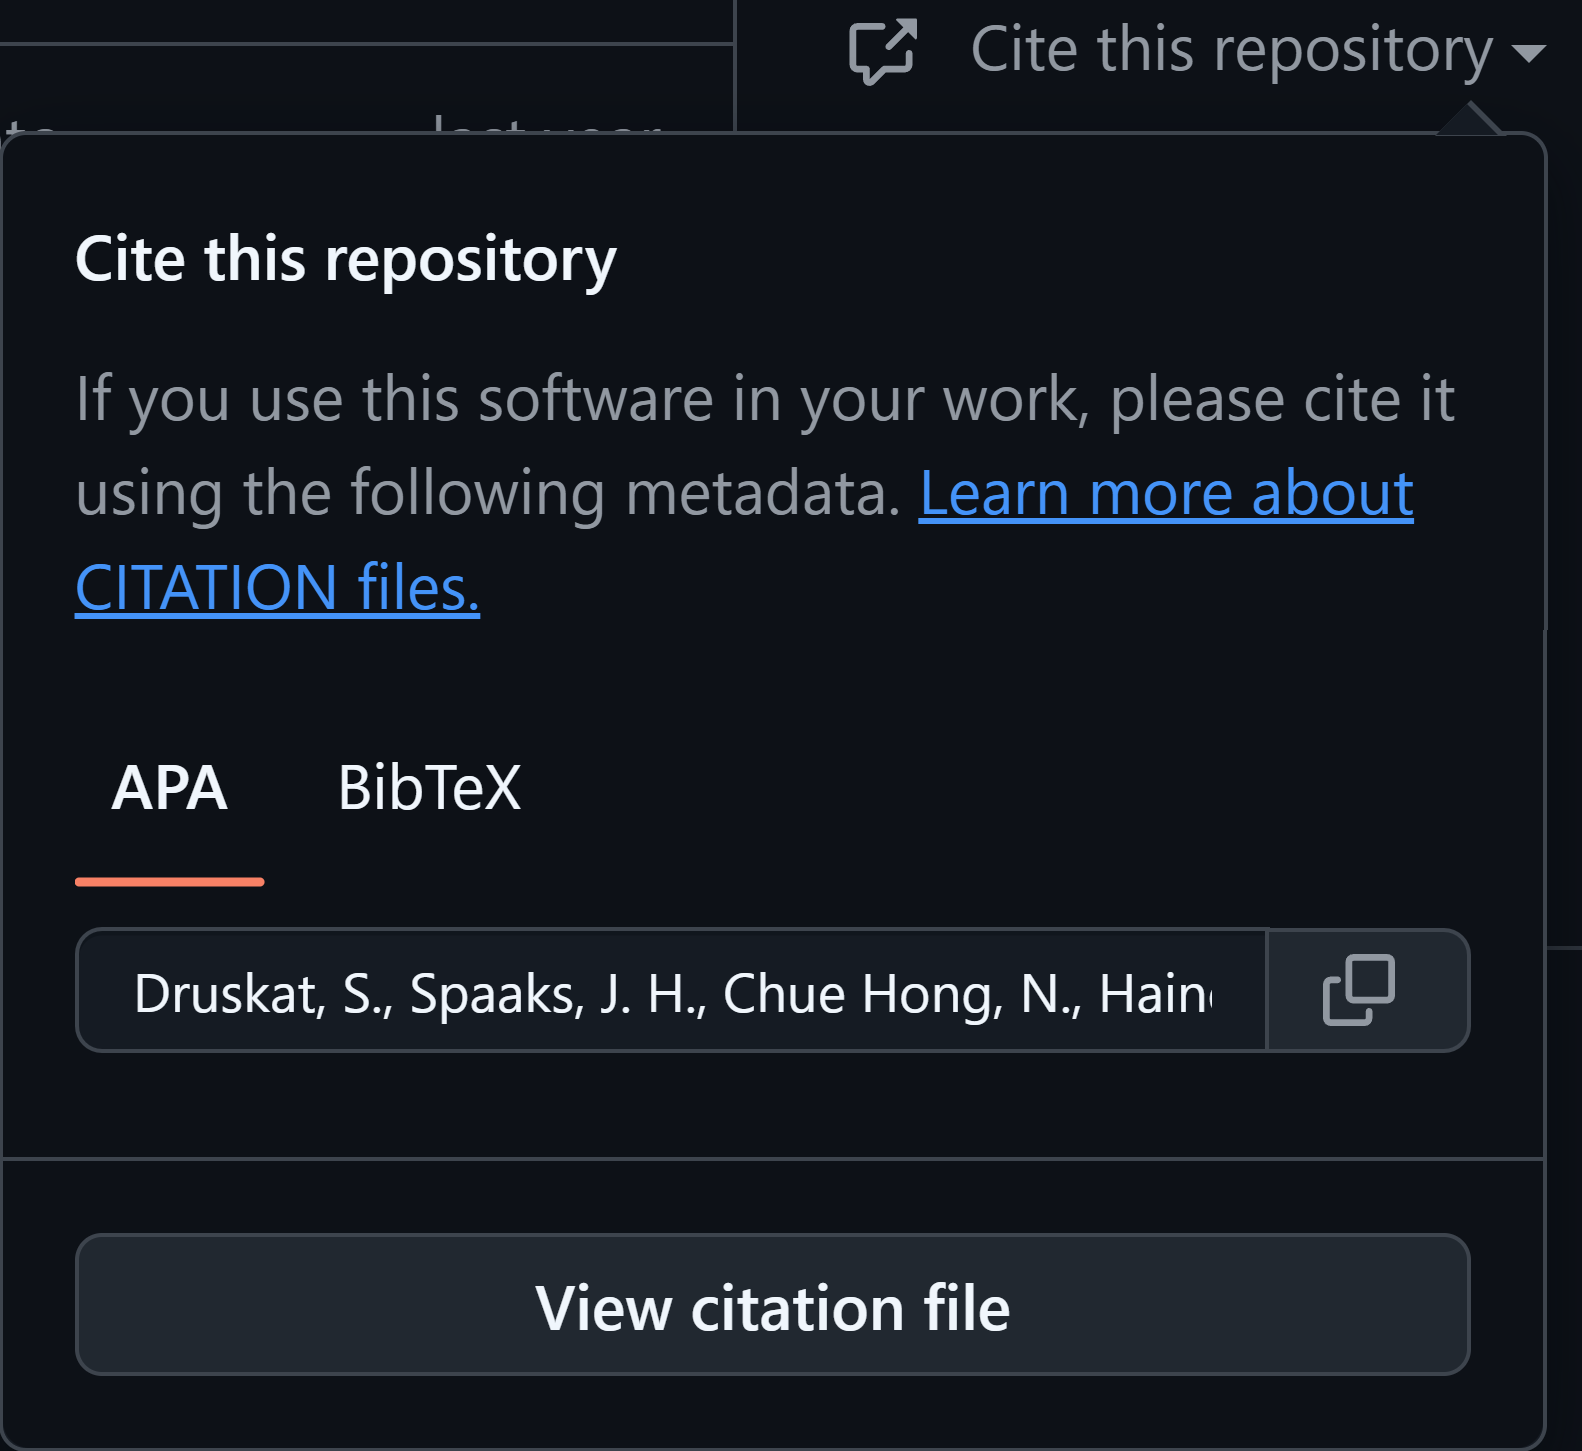
\includegraphics[width=0.5\textwidth]{bilder/GH_CFF_link.png}
    \end{center}
    \caption{GitHub-Repository mit \mintinline{text}{CITATION.cff}-Datei}
    \label{fig:gh_cff_link}
    \small
    Die Abbildung stellt den Link auf die \mintinline{text}{CITATION.cff}-Datei dar, wie ihn GitHub aktuell darstellt.
    Außerdem ist die Möglichkeit sichtbar, die Datei im \hologo{BibTeX}-Format und in der APA-Zitierweise zu kopieren \autocite{druskat_citation_2021-1}.
\end{figure}

In dem \gls{cff} existieren verschiedene Felder, welche für die Zitation von Software relevant sind.
Das wichtigste Feld ist das \emph{authors}-Feld, welches die Autoren der Software enthält und zwingend erforderlich ist.
In diesem Feld können die Autoren als Liste angegeben werden.
Ein Autor ist dabei entweder eine Person oder eine Entität.
Eine Entität kann beispielsweise eine Organisation sein.
Die Entität kann mit einem Namen mittels \emph{name} angegeben werden \autocite{druskat_citation_2021}.
Sie kann ebenfalls eine OORCID iD und eine E-Mail-Adresse enthalten.
Besonders wichtig für diese Arbeit ist die Referenz auf eine Person, da dies die einzige Information ist, welche aus Git extrahiert werden kann.
Eine Person enthält ebenfalls die genannten Werte einer Entität und wird jedoch über den Vor- und Nachname separiert mittels \emph{given-names} und \emph{family-names} angegeben.
Dadurch ist es möglich, die Personen von den Entitäten zu unterscheiden.

Ein weiteres Feld ist das \emph{preferred-citation}-Feld.
Mit diesem Feld ist es möglich, die Anerkennung für die Arbeit auf eine andere Arbeit zu übertragen \autocite{druskat_citation_2021}.
Ein Beispiel hierfür ist ein Paper über die Software, welches bevorzugt zitiert werden soll, anstelle der eigentlichen Software.
Hierbei können ebenfalls Personen und Entitäten angegeben werden.
Durch die Angabe einer \emph{preferred-citation} kann das Prinzip der Wichtigkeit vernachlässigt werden.
Auf dieses Verhalten wird in der Diskussion konkreter eingegangen.

Weitere in dieser Arbeit verwendete Felder sind \emph{type}, \emph{year}, \emph{month}, \emph{date-released}, \emph{date-published}, \emph{doi}, \emph{collection-doi} und \emph{identifiers}.
Das Feld \emph{type} ist zwingend erforderlich, hat jedoch als Standardwert \glqq software\grqq{}, sodass dies nicht angegeben werden muss.
Es gibt an, ob es sich um eine Software oder einen Datensatz handelt.
Dabei sind lediglich die Werte \glqq software\grqq{} oder \glqq dataset\grqq{} erlaubt.
Das Feld \emph{date-released} gibt an, wann die Software oder der Datensatz veröffentlicht wurde.
Das Feld \emph{doi} kann einen \glsdisp{doi}{Digitalen Objektbezeichner (DOI)} der Software oder des Datensatzes enthalten.
Mittels \emph{identifiers} können weitere Identifikatoren angeführt werden, wie z.~B. eine \gls{doi} oder eine URL, wobei die \emph{identifiers} mit einer Beschreibung erweitert werden können.
Die beschriebenen Felder können zusätzlich alle unter dem Feld \emph{preferred-citation} angegeben werden, um eine andere Arbeit zu referenzieren.

Die Felder \emph{year}, \emph{month} und \emph{date-published} können zusätzlich zu dem Feld \emph{date-released} unter dem Feld \emph{preferred-citation} angeführt werden, um das Jahr und das Datum der Veröffentlichung anzugeben.
Außerdem können weitere Typen mittels \emph{type} aufgeführt werden, wie beispielsweise \glqq thesis\grqq{} oder \glqq manual\grqq{}, sodass diese Arbeiten ebenfalls referenziert werden können.
Zusätzlich kann das Feld \emph{collection-doi} verwendet werden, um auf eine Sammlung von Arbeiten zu verweisen, die die Arbeit enthält.
Ein Beispiel einer \mintinline{text}{CITATION.cff}-Datei ist in \autoref{lst:cff_example} dargestellt.
Dabei wurde sich auf die beschriebenen und notwendigen Felder beschränkt.

\begin{listing}
    \inputminted{yaml}{../CITATION.cff}
    \caption{Beispiel einer \mintinline{text}{CITATION.cff}-Datei}
    \label{lst:cff_example}
    \small
    In dem Listing ist die \gls{cff}-Datei dieser Arbeit dargestellt. Dabei wurden primär Felder angegeben, welche in der Masterarbeit verwendet werden.
\end{listing}

\subsection{\hologo{BibTeX}}
\label{subsec:bibtex_format}
\hologo{BibTeX} ist eine Software, welche zur Erstellung von Literaturangaben und -verzeichnissen in \LaTeX{}-Dokumenten verwendet wird.
Außerdem existiert mit \hologo{BibTeX} ein gleichnamiges Format, welches in der \mintinline{text}{CITATION.bib}-Datei gespeichert wird und auf keinem anderen Format basiert.
\hologo{BibTeX} ist ein weit verbreiteter Standard und wird von vielen Autoren in der Wissenschaft verwendet.
Auf GitHub enthalten 2.144 Repositorys eine \mintinline{text}{CITATION.bib}-Datei (Stand 07.11.2024).
Das Format beschreibt die Zitation von Literatur und kann von Menschen und Maschinen gelesen werden.
Es beschränkt sich dabei nicht auf eine spezielle Art von Literatur, sondern kann für viele unterschiedliche Arten von Literatur verwendet werden.
Beispielsweise können Bücher und Masterarbeiten in \hologo{BibTeX} zitiert werden \autocite{patashnik_bibtexing_1988}.
Ein offizieller Literaturtyp für Software existiert nicht.
In der Datei können mehrere Einträge vorhanden sein, wobei jeder Eintrag eine Literaturangabe darstellt.

\hologo{BibTeX}-Dateien können von Menschen manuell erstellt und in das Repository eingebunden werden.
Außerdem existieren viele Literaturverwaltungsprogramme wie Zotero, welche \hologo{BibTeX}-Dateien erstellen und verarbeiten können \autocite{zotero_zotero_2024}.
Ebenfalls ist die Integration in andere Plattformen möglich, wie z.~B. in GitHub.
Hier wird die \mintinline{text}{CITATION.bib}-Datei auf der Repository-Startseite verlinkt, sie lässt sich jedoch im Gegensatz zu dem \gls{cff} nicht direkt kopieren oder in andere Formate umwandeln \autocite{github_about_2024-1}.

In dem \hologo{BibTeX}-Format existieren verschiedene Felder, welche für die Zitation von Literatur relevant sind.
Welche Felder zwingend erforderlich sind, hängt vom jeweiligen Literaturtyp ab.
Zudem sind die verfügbaren Felder ebenfalls vom Literaturtyp abhängig \autocite{patashnik_bibtexing_1988}.
In dieser Arbeit wird auf einige dieser Felder eingegangen, welche für die spätere Auswertung relevant sind.
Das wichtigste Feld ist das \emph{author}-Feld, welches die Autoren der Literatur enthält und zwingend erforderlich ist.
Die Vor- und Nachnamen der Autoren werden mit einem Komma separiert und mehrere Autoren werden über ein \glqq and\grqq{} getrennt.
Weitere Felder, welche für die Masterarbeit verwendet werden, sind \emph{year} und \emph{month}, welche das Jahr und den Monat der Veröffentlichung angeben.
Ein Beispiel einer \mintinline{text}{CITATION.bib}-Datei ist in \autoref{lst:bibtex_example} dargestellt.
Es ist zu erkennen, dass in dem \hologo{BibTeX}-Eintrag Informationen fehlen, welche in dem \gls{cff}-Eintrag vorhanden waren.
Dies liegt daran, dass in dem \hologo{BibTeX}-Eintrag nur eine Referenz auf die Masterarbeit möglich ist und nicht auf die entwickelte Software.

\begin{listing}
  \inputminted{text}{../CITATION.bib}
  \caption{Beispiel einer \mintinline{text}{CITATION.bib}-Datei}
  \label{lst:bibtex_example}
  \small
  In dem Listing ist die \hologo{BibTeX}-Datei dieser Arbeit dargestellt. Dabei wurden primär Felder angegeben, welche in der Masterarbeit verwendet werden.
\end{listing}

\section{Named Entity Recognition}
\label{sec:named-entity-recognition}

\section{Named Entity Disambiguation}
\label{sec:author-name-disambiguation}
% TODO ggf. noch weiter ausführen?
Die \gls{ned} ist ein automatischer Prozess, bei dem ein Name einer Entität einer gegebenen Datenmenge zugeordnet wird \autocites{cucerzan_large-scale_2007}{yamada_global_2022}.
Die Entitäten können beispielsweise durch die \gls{ner} extrahiert worden sein.
Dabei kann es dazu kommen, dass eine Entität mehrfach extrahiert wird und mehrfach in der Datenmenge vorhanden ist, jedoch mit anderen Bedeutungen.
In der natürlichen Sprachverarbeitung ist dies das Problem der Polysemie.
Es ist aber auch möglich, dass Personen mit dem gleichen Namen, sogenannte Namensvetter extrahiert werden, welche unterschieden werden müssen.
Dies beschreibt die Author name disambiguation, welche konkret individuelle Personen disambiguiert und ein Teil der \gls{ned} ist.
Diese Probleme kann die \gls{ned} mittels Modellen lösen, die die Entitäten anhand von Kontexten disambiguieren.
Beispiele für erkannte Entitäten sind \autocite{cucerzan_large-scale_2007}:

\begin{itemize}
  \item George W. Bush (George W. Bush)
  \item George Bush (George W. Bush)
  \item Bush (George W. Bush)
  \item Reggie Bush (Reggie Bush)
  \item Bush (Reggie Bush)
  \item Bush (Rock band)
\end{itemize}

In dem Beispiel ist die Entität dargestellt, gefolgt von der Entität in der Datenmenge, welche in Klammern steht.
Hierbei ist auffällig, dass Nennungen von \glqq Bush\grqq{} mehrfach vorkommen und durch den Kontext, in dem sie stehen, durch die \gls{ned} unterschieden werden müssen.

\gls{ned} wird in vielen Bereichen eingesetzt, wie z.~B. Textanalysen, semantische Suche und der Gruppierung von Software-Nennungen in wissenschaftlichen Arbeiten \autocites{cucerzan_large-scale_2007}{yamada_global_2022}{schindler_somesci-_2021}.
In dieser Masterarbeit kann die \gls{ned} verwendet werden, um Autoren aus verschiedenen Quellen miteinander abzugleichen.

Ähnlich zu der \gls{ner} gibt es für die \gls{ned} verschiedene Modelle.
Viele Modelle sind jedoch spezifisch auf einzelne Aufgabenbereiche trainiert.
Allgemeine Modelle sind primär für die Disambiguierung von Entitäten in Texten trainiert, welche in dieser Arbeit nicht immer vorhanden sind.
Ein Beispiel ist ein Modell von Yamade u.~a., welches Wörter, sowohl als auch Entitäten als Tokens erhält und diese mit Entitäten aus einem Text disambiguiert \autocite{yamada_global_2022}.

\section{Unscharfe Suche}
\label{sec:unscharfe-suche}
% TODO ggf. Levenshtein Distance und Damerau-Levenshtein-Distanz leicht erklären
% TODO ggf. noch weiter ausführen?
Die unscharfe Suche ist ein Verfahren, um ähnliche Zeichenfolgen zu finden, die sich in ihrer Schreibweise unterscheiden \autocite{hall_approximate_1980}.
Dieses Verfahren hat viele Anwendungsgebiete in der Informatik.
Ein Beispiel ist das Finden eines Personennamens in einem Index.
Falls der Name exakt in dem Index vorhanden ist, ist die Suche trivial.
Falls der Name unterschiedlich geschrieben ist, beispielsweise durch Abkürzungen oder Tippfehler, schlägt die triviale Suche fehl.
Die unscharfe Suche kann in diesem Fall helfen, den Namen dennoch zu finden.
Ein weiteres Anwendungsgebiet ist eine allgemeine Suche, beispielsweise von Produkten in einem Online-Shop.
Hierbei müssen auch Tippfehler berücksichtigt werden.

Die unscharfe Suche kann auf der Levenshtein-Distanz basieren \autocite{levenshtein_binary_1965}.
Als Ergebnis der unscharfen Suche wird in vielen Implementierungen die Distanz zwischen zwei Zeichenfolgen in Prozent angegeben.
Die Levenshtein-Distanz verwendet drei Arten von einzelzeichenbasierten Editieroperationen, um die Distanz zwischen zwei Zeichenfolgen zu berechnen.

\begin{enumerate}
    \item Einfügen eines Zeichens zur Zeichenfolge (Suhe \rightarrow{} Su\textbf{c}he)
    \item Löschen eines Zeichens aus der Zeichenfolge (Suche\textbf{e} \rightarrow{} Suche)
    \item Ersetzen eines Zeichens in der Zeichenfolge (S\textbf{i}che \rightarrow{} S\textbf{u}che)
\end{enumerate}

Zusätzlich zu der Levenshtein-Distanz existiert eine Erweiterung, die Damerau-Levenshtein-Distanz \autocite{damerau_technique_1964}.
Diese erweitert die Levenshtein-Distanz um eine vierte Editieroperation.
Mittels dieser vier Operationen werden ungefähr 80 \% der menschlichen Tippfehler abgedeckt \autocite{damerau_technique_1964}.

\begin{enumerate}
    \setcounter{enumi}{3}
    \item Vertauschen von zwei benachbarten Zeichen in der Zeichenfolge (Su\textbf{hc}e \rightarrow{} Su\textbf{ch}e)
\end{enumerate}

Eine Herausforderung bei der unscharfen Suche ist die Laufzeit.
Sie ist ungefähr proportional zum Produkt der beiden Zeichenfolgenlängen, wodurch eine unscharfe Suche nach langen Zeichenfolgen unpraktisch wird.
Eine weitere Herausforderung ist das Finden des richtigen Prozentsatzes, um die unscharfe Suche zu verwenden.
Ein zu hoher Prozentsatz führt dazu, dass die Suche zu viele Ergebnisse zurückgibt, während ein zu niedriger Prozentsatz dazu führt, dass die Suche zu wenige Ergebnisse zurückgibt.

Für die unscharfe Suche gibt es viele Implementierungen, die auf verschiedenen Algorithmen basieren.
Ein Programm, welches in Python implementiert ist, ist \emph{TheFuzz} \autocite{bachmann_thefuzz_2023}.
Das Programm basiert auf \emph{RapidFuzz}, welches die Levenshtein-Distanz in Python und C++ implementiert \autocites{bachmann_rapidfuzz_2023}.


\chapter{Methodik}
\label{chap:methodik}
% TODO Grafik hier einfügen vom Prozess
In diesem Kapitel wird beschrieben wie die Daten der einzelnen Quellen beschafft, abgeglichen und anschließend ausgewertet werden.
Die Datenbeschaffung wird in \autoref{sec:datenbeschaffung}, der Abgleich in \autoref{sec:abgleich} und die Auswertung in \autoref{sec:auswertung} beschrieben.

Die Datenbeschaffung in wurde in die einzelnen Quellen untergliedert.
Einige Methoden zur Datenbeschaffung sind dabei ähnlich, worauf im konkreten Fall eingegangen wird.
Diese werden jedoch nicht doppelt erläutert.

Der Abgleich findet jeweils zwischen Git und einer weiteren Quelle statt.
Es existiert kein Abgleich zwischen einzelnen Quellen wie den Daten aus \gls{pypi} und der Beschreibung.
Der Abgleich wird in jeder Datenbeschaffung außer der von Git automatisch durchgeführt.
Die Ergebnisse des Abgleichs werden in einer CSV-Datei gespeichert.
Allgemeine Daten, beispielsweise ob die Quelle valide ist, werden ebenfalls in einer CSV-Datei gespeichert.
Falls in einer Quelle keine Daten vorhanden sind, wird keine CSV-Datei für diese erstellt.

Sämtliche Ergebnisse werden, falls verfügbar, zu verschiedenen Zeitpunkten in denen Änderungen an der Quelle vorgenommen wurden ermittelt und gespeichert.
Falls aus der Quelle verschiedene Zeitpunkte der Änderungen vorliegen, wird der Abgleich mit Git jeweils mit der neusten Version durchgeführt und mit der Version, welche zu dem Zeitpunkt der Änderung in der Quelle vorhanden war.
Dadurch entstehen für ein Paket mehrere Dateien, welche unterschiedliche Werte enthalten.
Es entsteht die in \autoref{fig:datenbeschaffung_ergebnisse} dargestellte Ordnerstruktur, welche die Ergebnisse der Datenbeschaffung darstellt.

\begin{figure}
    \centering
    \dirtree{%
        .1 /\DTcomment{Wurzelverzeichnis}.
        .2 20210819\_161452-0400\_bib\_authors.csv\DTcomment{\hologo{BibTeX} Autoren abgeglichen mit den Git Werten zu diesem Zeitpunkt}.
        .2 20210819\_161452-0400\_bib\_authors\_new.csv\DTcomment{\hologo{BibTeX} Autoren abgeglichen mit den Git Werten zum neusten Zeitpunkt}.
        .2 20210819\_161452-0400\_git\_contributors.csv\DTcomment{Git Autoren zu diesem Zeitpunkt}.
        .2 bib.csv\DTcomment{Allgemeine informationen zur \hologo{BibTeX}-Datei zu allen Zeitpunkten z. B. eingetragene DOI}.
        .2 git\_contributors.csv\DTcomment{Git Autoren zum neusten Zeitpunkt}.
        .2 pypi\_maintainers.csv\DTcomment{\gls{pypi} Maintainer}.
        .2 python\_authors.csv\DTcomment{In Python angegebene Autoren}.
    }
    \caption{Ergebnisse der Datenbeschaffung}
    \label{fig:datenbeschaffung_ergebnisse}
    \small
    Die Abbildung stellt einen Ausschnitt der CSV-Dateien der Datenbeschaffung dar.
\end{figure}

Der Prozess findet für jedes zu untersuchende Paket statt.
Die Pakete werden dabei aus dem \gls{pypi} und dem \gls{cran} Software-Verzeichnis entnommen.
Es werden die Top 100 \gls{pypi} Pakete im August 2024 untersucht, welche am häufigsten heruntergeladen wurden \autocite{kemenade_hugovktop-pypi-packages_2024}.
Von \gls{cran} werden die Top 100 meist heruntergeladenen Pakete im Zeitraum von 02.08.2024 bis 31.08.2024 untersucht \autocite{csardi_r-hubcranlogsapp_2024}.
Außerdem werden die Top 100 Pakete, welche eine \gls{cff}-Datei in GitHub haben untersucht.
Die Top 100 werden dabei durch die Anzahl der Sterne auf GitHub definiert.
Die Liste wurde am 19.10.2024 erstellt.
In der Liste sind Pakete enthalten, welche nicht im \gls{pypi} oder \gls{cran} verfügbar sind.
Diese Pakete werden nicht betrachtet.

Die Ergebnisse werden in drei Ordnern gespeichert jeweils für \gls{pypi} \gls{cran} und \gls{cff}.
In jedem Ordner sind jeweils Unterordner für die einzelnen Pakete.
Diese Daten werden für die anschließende Auswertung in \autoref{sec:auswertung} verwendet.
Hier werden die Ergebnisse der Abgleiche ausgewertet und zusammengefasst, um über alle Pakete hinweg Aussagen treffen zu können.
Die Datenbeschaffung, der Abgleich und die Auswertung sind in Python programmiert und verwenden \gls{oss} auf welche in den jeweiligen Abschnitten eingegangen wird.
Über alle Abschnitte hinweg wird Pandas in der Version 2.2.2 verwendet, um die Tabellen zu erstellen und zu verarbeiten \autocite{the_pandas_development_team_pandas-devpandas_2024}.

\section{Datenbeschaffung}
\label{sec:datenbeschaffung}
\subsection{Git}
\label{subsec:git}
% TODO Beschreiben wie die Commits gezählt wurden.
\subsection{PyPi}
\label{subsec:pypi}
% TODO auf verifizierte PyPi Nutzer eingehen
% Checken was verifizierte Nutzer im PyPi Universum bedeutet. Sind es nur verifizierte User die z.B. eine E-Mail hinterlegt haben oder sind es Nutzer die an dem Projekt arbeiten und von PyPi verifiziert sind? Falls es mehrwert hat diese Daten ebenfalls automatisch abfragen und auch in der MA beschreiben, was es nun ist und warum es Mehrwert hat oder auch nicht.
% In MA beschreiben, warum oder warum nicht Mehrwert (PyPi Verifizierte Nutzer)
% Verifizierte Daten sind Daten, welche PyPi als "richtig" ansieht. Aktuell ist es im Prozess, dass immer mehr Daten diesen Status erreichen. Aktuell können nur der Owner und Maintainer diesen Status erreichen. Verifizierte Maintainer sind dabei Personen, welche bei PyPi registriert sind und dem Projekt zugeordnet sind. Also das Projekt auf PyPi verwalten können.
% https://github.com/pypi/warehouse/issues/8635
% https://github.com/pypi/warehouse/issues/15903
% https://peps.python.org/pep-0740/
% https://github.com/pypi/warehouse/issues/15871 (Roadmap Pep 740)
% Aktuell gibt es noch keinen weg die verified details über die API zu beziehen (https://github.com/pypi/warehouse/issues/14799) aus diesem Grund muss es aus dem HTML code extrahiert werden.
% Verifizierte "Maintainer" in PyPi sind Personen, welche neue Releases veröffentlichen dürfen (https://github.com/pypi/warehouse/issues/13366)
% Die nicht verifizierten Daten stammen aus der Python toml
% Es existiert aktuell keine API für user (https://github.com/pypi/warehouse/issues/15769) aus diesem Grund muss ich die aus dem HTML besorgen.
\subsection{CRAN}
\label{subsec:cran}
\subsection{Beschreibung}
\label{subsec:beschreibung}
% TODO Es werden alle Namen ausgegeben aber auch eben solche, die gar nichts mit dem Paket zu tun haben wie im fall von highr für CRAN: "Provides syntax highlighting for R source code. Currently it supports LaTeX and HTML output. Source code of other languages is supported via Andre Simon's highlight package (https://gitlab.com/saalen/highlight)." Es gibt noch weitere Beispiele z.B. in CRAN magrittr
\subsection{Citation File Format}
\label{subsec:cff}
\subsection{BibTeX}
\label{subsec:bibtex}
 % 12.5 Seiten
\section{Abgleich}
\label{sec:abgleich}
% TODO Grafik erstellen, die das ganze nochmal visualisiert
In diesem Abschnitt wird beschrieben, wie die Autoren aus den unterschiedlichen Quellen, welche in der Datenbeschaffung erläutert wurden, abgeglichen werden.
Dabei werden jeweils die Git Autoren mit den Autoren aus den anderen Quellen abgeglichen.
Für diesen Prozess wird keine \gls{ned} verwendet, sondern ein eigener Algorithmus, welcher auf die Daten angepasst ist.
Dieser wurde entwickelt, indem die Autoren, welche durch die Datenbeschaffung erhalten wurden, in den Paketen eingesehen wurden.
So wurde durch viel Probieren eine möglichst gute Lösung gefunden, welche im Folgenden beschrieben wird.
Dies führt allerdings dazu, dass der entwickelte Algorithmus nicht in der Lage ist zwei Autoren mit dem gleichen Namen zu unterscheiden, falls keine weiteren Daten wie eine E-Mail vorhanden sind.

Als Eingabe erhält der Algorithmus eine Liste von Autoren, welche in einer Quelle (z. B. \gls{cff}) gefunden wurden und jeweils die Liste der Git Autoren für das zu untersuchende Paket.
In der Datenbeschaffung wurde gezeigt, dass die Autoren aus den Quellen einen Namen, eine E-Mail und einen Benutzernamen enthalten können, abhängig von der Quelle.
In dem Algorithmus wird ermittelt, wie viele von den Daten vorhanden sind, um im Verlauf einen Score berechnen zu können wie viele der Daten übereinstimmen.
Falls Beispielsweise die Quelle \gls{cff} ist, kann der Name und die E-Mail vorhanden sein.
Dadurch ergibt sich, dass maximal zwei Daten mit denen von Git übereinstimmen können.
Falls die Quelle die Beschreibung ist, ist maximal eine Übereinstimmung möglich.
Diese Daten werden für den Abgleich verwendet.
Die eingegebene Liste der Git Autoren muss für den Algorithmus nach der Anzahl der Commits sortiert sein, da der Algorithmus Personen mit den meisten Commits bevorzugt.
Anschließend wird jeder Autor aus der Quelle mit jedem Git Autor abgeglichen.
Dabei werden alle Werte in Kleinbuchstaben umgewandelt, um zu gewährleisten, dass auch bei unterschiedlicher Schreibweise eine Übereinstimmung gefunden werden kann.

Dabei wird so vorgegangen, dass die Daten, welche vorhanden sind, zum Vergleich herangezogen werden.
Falls der Name vorhanden ist, wird dieser mit dem Namen des Git Autors über das Keyword \emph{in} in Python verglichen.
Dieses sorgt dafür, dass nur ein Teil der Zeichenkette in der anderen Zeichenkette vorhanden sein muss.
Außerdem wird die andere Richtung ebenfalls probiert.
Zusätzlich wird das Programm \emph{thefuzz} in der Version 0.22.1 verwendet, um eine unscharfe Suche zu ermöglichen.
Hierbei wird der Name des Autors aus der Quelle mit dem Namen des Git Autors verglichen und auf eine Übereinstimmung von 80 \% oder mehr geprüft.
Die Datenbeschaffung hat gezeigt, dass die Namen der Autoren manchmal Klammern enthalten, welche den beschriebenen Abgleich stören.
Aus diesem Grund wird der zuvor beschriebene Abgleich erneut durchgeführt, wobei die Klammern in dem Namen entfernt worden sind.

Falls eine E-Mail vorhanden ist, wird diese mit der E-Mail des Git Autors über das Keyword \emph{in} verglichen.
Die andere Richtung wird ebenfalls probiert, also die E-Mail des Git Autors mit der E-Mail des Autors aus der Quelle über das Keyword \emph{in} zu vergleichen.
Zusätzlich wird erneut die unscharfe Suche zwischen der E-Mail des Autors aus der Quelle und der E-Mail des Git Autors durchgeführt und auf eine Übereinstimmung von 80 \% oder mehr geprüft.
Falls kein Abgleich über den Namen stattgefunden hat, wird ein Vergleich zwischen der E-Mail des Autors aus der Quelle und dem Namen des Git Autors über das Keyword \emph{in} durchgeführt.
Außerdem wird der Abgleich erneut über die unscharfe Suche mit einer Übereinstimmung von 80 \% oder mehr durchgeführt.
Dies führt dazu, dass weitere Übereinstimmungen gefunden werden können, falls der Name zu keiner Übereinstimmung geführt hat.
Dies liegt daran, dass viele Autoren in ihrer E-Mail-Adresse ihren Namen enthalten haben.
Außerdem hat die Datenbasis gezeigt, dass es vorkommt, dass in dem E-Mail Feld keine E-Mail angegeben wurde, sondern ein Name und als Resultat das Namensfeld nicht ausgefüllt wurde.

Falls ein Benutzername vorhanden ist, wird dieser mit der E-Mail des Git Autors verglichen, da aus den Git Daten kein Benutzername extrahiert werden kann.
Dies ist möglich, da viele Autoren für ihren Benutzernamen den lokal Teil der E-Mail verwenden.
Für den Vergleich wird die E-Mail, falls sie ein @ Symbol enthält, an dieser Stelle getrennt.
Anschließend wird der vordere lokale Teil für den Vergleich mit dem Benutzernamen aus der Quelle verwendet.
Dabei wird der Vergleich erneut über das Keyword \emph{in} in beiden Richtungen durchgeführt.
Außerdem wird über die unscharfe Suche mit einer Übereinstimmung von 80 \% oder mehr geprüft, ob eine Übereinstimmung gefunden wurde.
Dieser Prozess wird ebenfalls erneut für den Domain-Teil der E-Mail durchgeführt, sodass dieser ebenfalls mit dem Benutzernamen verglichen wird.

Falls keiner dieser drei Vergleiche zu einem Erfolg geführt hat, wird der Name des Autors mit dem lokalen Teil der E-Mail des Git Autors über die unscharfe Suche verglichen.
Dabei muss erneut eine Übereinstimmung von 80 \% oder mehr vorhanden sein, um den Vergleich als gelungen zu bewerten.

Anschließend wird der Score berechnet.
Dabei wird die Anzahl der Übereinstimmungen durch die Anzahl der maximal möglichen Übereinstimmungen geteilt.
Falls beispielsweise der Name und die E-Mail vorhanden sind, sind maximal zwei Übereinstimmungen möglich.
Bei einer Übereinstimmung des Namens und die E-Mail ergibt sich ein Score von 1.
Falls nur der Name übereinstimmt, ergibt sich ein Score von 0,5.
Dieser Score wird für jeden Autor aus der Quelle mit jedem Git Autor berechnet und in der Tabelle der Autoren aus der Quelle gespeichert.
Anschließend wird der Autor aus der Quelle mit dem Git Autor mit dem besten Score ausgewählt.
Falls es zwei Einträge in der Git Liste gibt, welche einen gleichen Score erreichen, wird der Autor ausgewählt, welcher die meisten Commits hat.
Außerdem wird der Rang, welcher der Autor in der Git Autoren Liste belegt zurückgegeben.
Als Ergebnis des Abgleichs werden alle Autoren aus der Quelle, welche in den Algorithmus eingegeben wurde, zurückgegeben.
Die Autoren werden dabei mit den Ergebnissen des Abgleichs verbunden, welche in \autoref{tab:abgleich_felder} dargestellt sind.
Das Ergebnis des Abgleichs ist in \autoref{tab:abgleich_felder} dargestellt.
Falls kein Abgleich für einen Autor möglich war, werden die Felder für diesen Autor leer gelassen.
Anschließend wird das Ergebnis nach dem Rang sortiert, also nach der Anzahl der Commits, welche der Autor hat.
 % 2 Seiten
\section{Auswertung}
\label{sec:auswertung}
In diesem Abschnitt wird beschrieben, wie die Daten aus dem \autoref{sec:datenbeschaffung} ausgewertet werden.
Dabei wird der Abschnitt aufgeteilt in die Aggregierung der Daten, welche zuvor beschrieben wurden und anschließend wird kurz auf die Darstellung der aggregierten Daten eingegangen.

Die Auswertung der Daten erfolgt erneut mittels Python.
Für die Auswertung werden alle Daten verarbeitet, welche durch die Datenbeschaffung gesammelt wurden.
Einzige Ausnahme ist, dass immer die Dateien mit der \emph{new} Endung betrachtet werden.
Dies liegt daran, dass die Auswertung aktuell nur auf den neuesten Git-Daten durchgeführt wird und die Git-Daten zu den jeweiligen Zeitpunkten der Änderung nicht betrachtet werden.
Außerdem ist darüber ein Abgleich zwischen den Git-Autoren und den Autoren aus den anderen Quellen möglich.
Aber auch ein Abgleich zwischen den einzelnen Quellen ist möglich, da die Autoren in der neuesten Version immer die gleichen Git-Daten wie beispielsweise die gleiche Anzahl an Commits in allen Quellen haben.
Der Abgleich der Autoren ist hierbei nur möglich, falls in der Datenbeschaffung die Autoren abgeglichen werden konnten.

Falls ein Abgleich zwingend erforderlich ist, beispielsweise bei der Untersuchung, wie lange ein Autor durchschnittlich in einer Quelle genannt ist, wird ein einfacher Vergleich des Namens über die Quelle durchgeführt.
Dieser Vergleich ist jedoch nicht immer korrekt, da beispielsweise Namensänderungen in den Quellen so nicht berücksichtigt werden können, falls kein Abgleich in der Datenbeschaffung möglich war.

Das Skript ist so aufgebaut, dass nicht alle Daten auf einmal geladen werden, sondern jede Datei einzeln geladen und verarbeitet wird.
Dies bietet den Vorteil, dass auch mit weniger Arbeitsspeicher gearbeitet werden kann und die Daten nicht alle auf einmal im Arbeitsspeicher gehalten werden müssen.
Jedoch birgt dies auch Nachteile, beispielsweise dass zu keinem Zeitpunkt bekannt ist, wie viele Autoren maximal in einer Quelle vorkommen.
Diese Information ist erst vorhanden, wenn alle Daten vollständig verarbeitet worden sind.

Zusätzlich ist die Aggregierung der Daten unterteilt in die Aggregierung der vollständigen Daten und die Aggregierung der neuesten Daten.
In der vollständigen Datenverarbeitung werden Ergebnisse extrahiert, die die gesamte Historie der Daten betrachten.
Hier werden alle Daten mit ihren Zeitstempeln verarbeitet.
In der neuesten Datenverarbeitung werden nur die Daten betrachtet, die auf dem neuesten Stand der untersuchten Software sind.
Dabei wird jeweils die neueste Datei in den Quellen mithilfe des Zeitstempels ausgewählt und anschließend verarbeitet.
In diese beiden Kategorien ist das \autoref{chap:ergebnisse} ebenfalls unterteilt.
 % 2 Seiten

\chapter{Ergebnisse}
\label{chap:ergebnisse}
% TODO ggf. noch weitere full cff graphen hinzufügen
% TODO ggf. noch auf die Daten in #20 eingehen? Das dann mit und ohne Zeitverlauf?
In diesem Kapitel werden die Ergebnisse der Masterarbeit präsentiert.
Das Kapitel ist in zwei Abschnitte unterteilt.
Zum einen werden die Ergebnisse der Gegenwart in \autoref{sec:neuste_ergebnisse} präsentiert.
Hierbei werden die jeweils neuesten Dateien aus der Datenbeschaffung untersucht und Statistiken aufgeführt, welche in Verbindung mit diesen Daten stehen.
Zum anderen werden die Ergebnisse mit Zeitverlauf in \autoref{sec:gesamtheit_ergebnisse} präsentiert.
Hierbei werden die Dateien aus der Datenbeschaffung in allen Versionen analysiert.
Durch die Betrachtung aller Versionen können Veränderungen über die Zeit aufgezeigt werden.
In dem \autoref{sec:neuste_ergebnisse} wird zu Beginn auf die Statistiken des Abgleichs eingegangen und präsentiert, wie genau der Abgleich durchgeführt wurde.
Der Abgleich hat einen direkten Einfluss auf viele weitere Statistiken.

Die benötigten Daten für die Untersuchungen wurden in der Zeitspanne September 2024 bis November 2024 beschafft.
Dies liegt daran, dass die Repositorys lokal gespeichert werden und bei der Entwicklung der Arbeit die Daten nicht erneut beschafft werden mussten.
Die Daten einer Liste wurden jeweils an einem Tag beschafft, um eine Vergleichbarkeit zu gewährleisten.
In dem gesamten Kapitel wird \emph{matplotlib} in der Version 3.9.2 verwendet, um die Grafiken zu erstellen \autocite{hunter_matplotlib_2007}.

\section{Ergebnisse der Gegenwart}
\label{sec:neuste_ergebnisse}
Da die Ergebnisse der Masterarbeit direkt abhängig von der Qualität des Abgleichs sind, wurde diese untersucht.
Dies wurde auf zwei Arten durchgeführt.
Zum einen wurde automatisch die Anzahl der abgeglichenen und der nicht abgeglichenen Autoren untersucht.
Zum anderen wurden manuell für eine ausgewählte Menge an Personen die Ergebnisse händisch überprüft.
Es wurde in beiden Fällen die Überprüfung ausschließlich auf den neuesten Versionen der Daten durchgeführt.

Die automatische Überprüfung erfolgt bei der Auswertung der Daten aus der Datenbeschaffung.
Dabei wird für jede Liste und für jede Quelle z. B. \gls{cff} die Anzahl der abgeglichenen Autoren und der insgesamt vorhandenen Autoren ermittelt.
Hierbei wurde die gesamte Menge an Autoren betrachtet.
Die Ergebnisse für die Listen \gls{pypi} \gls{cff} und \gls{cran} \gls{cff} sind in \autoref{tab:matching_results_auto} dargestellt.
Für die weiteren Listen sind die Ergebnisse in \autoref{tab:matching_results_auto_anhang} zu finden.

\begin{table}
    \begin{tabularx}{\textwidth}{XR{3.8cm}R{3.8cm}}
        \toprule
        \textbf{Quelle}              & \textbf{\gls{pypi} \gls{cff}} & \textbf{\gls{cran} \gls{cff}} \\ \midrule
        \gls{cran} Autoren           &                               & 204/238 (85.71 \%)            \\
        \gls{cran} Maintainer        &                               & 99/100 (99.00 \%)             \\
        Beschreibung                 & 580/1070 (54.21 \%)           & 21/80 (26.25 \%)              \\
        README                       & 868/1396 (62.18 \%)           & 143/1008 (14.19 \%)           \\
        \gls{cff}                    & 477/598 (79.77 \%)            & 184/233 (78.97 \%)            \\
        \gls{cff} preferred citation & 294/380 (77.37 \%)            & 109/136 (80.15 \%)            \\
        \gls{pypi} Maintainer        & 206/228 (90.35 \%)            &                               \\
        Python Autoren               & 105/131 (80.15 \%)            &                               \\
        Python Maintainer            & 15/25 (60.00 \%)              &                               \\
        \hologo{BibTeX}              & 0/1 (0.00 \%)                 &                               \\ \midrule
        Summe                        & 2545/3829 (66.47 \%)          & 760/1795 (42.34 \%)           \\
        \bottomrule
    \end{tabularx}
    \caption{Automatische Ergebnisse des Abgleichs}
    \label{tab:matching_results_auto}
    \small
    In der Tabelle sind die Ergebnisse des automatischen Abgleichs für die Listen \gls{pypi} \gls{cff} und \gls{cran} \gls{cff} dargestellt. Die Werte geben an, wie viele der genannten Autoren in den Git-Repositorys gefunden wurden.
\end{table}

In den Ergebnissen ist auffällig, dass die Autoren in der README-Datei und in der Beschreibung der Pakete am schlechtesten abgeglichen werden konnten.
Dies liegt daran, dass hierbei die \gls{ner} verwendet wurde und diese nicht immer korrekt arbeitet.
Hierbei kommt es häufig vor, dass Entitäten erkannt werden, welche keine Person darstellen.
Außerdem werden Personen mit weiteren Zusätzen wie z. B. dem Anfang einer Internetadresse zurückgegeben, was den Abgleich erschwert.
Zusätzlich werden in der README und der Beschreibung häufig Personen genannt, welche z. B. Vorarbeit für die Software geleistet haben, aber in der Software selbst keinen Code beigetragen haben.
Diese Personen können nicht abgeglichen werden.
Die Python Maintainer konnten ebenfalls schlecht abgeglichen werden, da viele Pakete in diesem Feld keine Personen, sondern Organisationen nennen.

Allgemein bietet dieses Vorgehen keine Aussage darüber, ob die Personen nicht abgeglichen worden sind, weil sie keinen Code beigetragen haben oder weil sie nicht gefunden wurden.
Zudem werden Personen, welche fälschlicherweise mit einer anderen Person abgeglichen wurden, in diesem Verfahren als gut bewertet.
Um diese Fälle ebenfalls betrachten zu können, wurde manuell eine Auswahl an Autoren überprüft.
Es wurden nicht alle Autoren überprüft, da dies den zeitlichen Rahmen der Arbeit gesprengt hätte.
Aus diesem Grund wurden die Autoren für jedes Paket und jede Quelle zufällig neu angeordnet und gespeichert.
Anschließend wurden jeweils die ersten beiden Autoren anhand von vier Kriterien überprüft.
Falls nur ein Autor in einer Quelle genannt wurde, wurde nur dieser überprüft.
Jeder Autor wurde einer der vier Kategorien \glqq richtig positiv (TP)\grqq{}, \glqq falsch negativ (FN)\grqq{}, \glqq falsch positiv (FP)\grqq{} oder \glqq richtig negativ (TN)\grqq{} zugeordnet.
Ein Autor ist als richtig positiv klassifiziert worden, falls er richtig zugeordnet wurde.
Falls der Autor mehrfach in der Git-Autorenliste vorkommt, wurde der Autor als richtig positiv klassifiziert unabhängig davon, mit welchem von den doppelten Einträgen der Autor zugeordnet wurde.
Aus diesen Daten wurde der F1-Score berechnet.

Außerdem wurde angegeben, ob es sich um keine Person handelt, sondern z. B. um eine Organisation.
In diesen Fällen wurde der Eintrag dennoch in eine der vier Kategorien eingeteilt, wobei primär die Kategorie FP verwendet wurde, falls es eine Zuordnung gab.
Falls die Zuordnung allerdings mit einem Git-Autor erfolgt ist, welcher beispielsweise ein Bot der Organisation ist, wurde der Eintrag als TP eingeteilt, da es keinen Mechanismus in der Datenbeschaffung gibt, welcher Personen von nicht Personen unterscheiden kann.
Es wurde lediglich in der Datenbeschaffung darauf geachtet, möglichst keine Quellen zu berücksichtigen, welche keine Personen enthalten.
Die Ergebnisse für alle Listen zusammen sind in \autoref{tab:matching_results_manual} eingetragen.
Die Ergebnisse für die einzelnen Listen sind in den Tabellen \ref{tab:cran_matching_results_manual_anhang}, \ref{tab:pypi_matching_results_manual_anhang}, \ref{tab:cff_matching_results_manual_anhang}, \ref{tab:pypi_cff_matching_results_manual_anhang} und \ref{tab:cran_cff_matching_results_manual_anhang} dargestellt.
% TODO weitere Tabellen im Anhang referenzieren
% TODO eins zwei beispiele aus der Tabelle geben
% TODO auf eins zwei besonderheiten in der Tabelle eingehen z.B. schlechte werde in readme und beschreibung
% TODO auf die besonderheit eingehen, dass bei pypi super viele nicht personen in den Autorenlisten sind
% TODO confusion matrix und f1 score für alle listen zusammen (addiert) angeben diese hier zeigen und alle anderen im Anhang referenzieren.

\begin{table}
    \begin{tabularx}{\textwidth}{XR{.7cm}R{.7cm}R{.7cm}R{.7cm}R{2.8cm}R{2cm}}
        \toprule
        \textbf{Quelle} & \textbf{TP} & \textbf{FN} & \textbf{FP} & \textbf{TN} & \textbf{Keine Person} & \textbf{F1-Score} \\ \midrule
        Beschreibung                 & & & & & & \\
        README                       & & & & & & \\
        \gls{cff}                    & & & & & & \\
        \gls{cff} preferred citation & & & & & & \\
        \gls{pypi} Maintainer        & & & & & & \\
        Python Autoren               & & & & & & \\
        Python Maintainer            & & & & & & \\
        \gls{cran} Autoren           & & & & & & \\
        \gls{cran} Maintainer        & & & & & & \\
        \hologo{BibTeX}              & & & & & & \\ \midrule
        Summe                        & & & & & & \\
        \bottomrule
    \end{tabularx}
    \caption{Manuelle Ergebnisse des Abgleichs für alle Listen zusammen}
    \label{tab:matching_results_manual}
    \small
    In der Tabelle sind die Ergebnisse des manuellen Abgleichs für alle Listen eingetragen. Dabei wurde für jede Quelle die Anzahl der richtig positiven (TP), falsch negativen (FN), falsch positiven (FP) und richtig negativen (TN) Autoren ermittelt. Zusätzlich wurde angegeben, ob es sich um keine Person handelt und der F1-Score berechnet.
    In der Tabelle sind die Ergebnisse des manuellen Abgleichs für alle Listen. Dabei wurde für jede Quelle die Anzahl der richtig positiven (TP), falsch negativen (FN), falsch positiven (FP) und richtig negativen (TN) Autoren ermittelt. Zusätzlich wurde angegeben, ob es sich um keine Person handelt und der F1-Score berechnet.
\end{table}

Aus den gesammelten Daten wurden weitere Statistiken berechnet.
Dabei muss berücksichtigt werden, dass einige Statistiken auf dem Abgleich basieren und somit nur so gut sind, wie der Abgleich durchgeführt wurde.
Außerdem basieren einige Statistiken auf den Metriken der Commits und geänderten Zeilen.
Die Abbildung \autoref{fig:commits_vs_changed_lines} stellt das Verhältnis der Commits und der geänderten Zeilen für die Autoren in den Paketen der Listen \gls{pypi} \gls{cff} und \gls{cran} \gls{cff} dar.
Für die anderen Listen sind die Ergebnisse in \autoref{fig:commits_vs_changed_lines_anhang} dargestellt.
Ein Punkt stellt dabei einen Autor dar.
Es ist zu erkennen, dass einige Autoren nur einen Commit getätigt haben und dabei viele Zeilen geändert haben.
Beispielsweise hat der Autor François Lagunas in dem Paket \emph{huggingface/datasets} lediglich einen Commit getätigt, aber dabei ungefähr 29.000 Zeilen hinzugefügt.
Inhalt sind in diesem konkreten Fall automatisch generierte README-Dateien für Datensätze, welche zuvor gefehlt haben.

\begin{figure}
    \begin{subfigure}{.5\textwidth}
        \centering
        \includesvg[width=.95\linewidth,inkscapelatex=false]{bilder/commits_vs_changed_lines/commits_vs_changed_lines_pypi_cff.svg}
        \caption{\gls{pypi} \gls{cff}}
        \label{fig:commits_vs_changed_lines_pypi_cff}
    \end{subfigure}%
    \begin{subfigure}{.5\textwidth}
        \centering
        \includesvg[width=.95\linewidth,inkscapelatex=false]{bilder/commits_vs_changed_lines/commits_vs_changed_lines_cran_cff.svg}
        \caption{\gls{cran} \gls{cff}}
        \label{fig:commits_vs_changed_lines_cran_cff}
    \end{subfigure}
    \caption{Commits und geänderte Zeilen gegenübergestellt}
    \label{fig:commits_vs_changed_lines}
    \small
    Die Abbildungen zeigen für die Autoren in den Paketen in den Listen \gls{pypi} \gls{cff} und \gls{cran} \gls{cff} die Anzahl der Commits gegenüber der Anzahl der geänderten Zeilen. Die x-Achse stellt die Anzahl der Commits dar und die y-Achse die Anzahl der geänderten Zeilen. Es wird eine logarithmische Skalierung verwendet.
\end{figure}

Die \autoref{fig:common_authors} zeigt den Anteil der Top-Git-Autoren in den einzelnen Quellen, wie beispielsweise der \gls{cff}.
Dabei werden mehrere Abbildungen für die unterschiedlichen untersuchten Listen dargestellt.
In der konkreten Abbildung sind die Listen \gls{pypi} \gls{cff} und \gls{cran} \gls{cff} dargestellt.
Die Abbildungen für die weiteren Listen sind in \autoref{fig:common_authors_anhang} dargestellt.
Außerdem werden für jede Liste zwei unterschiedliche Abbildungen dargestellt.
Die eine Abbildung bemisst die Top-Git-Autoren an der Anzahl der Commits und die jeweils andere an der Anzahl der geänderten Zeilen.
Falls beispielsweise der Autor mit den meisten Commits in einer Quelle z. B. \gls{cff} genannt wird und die Autoren an den Commits bemessen werden und zusätzlich nur der Top-Autor betrachtet wird, so wird in der Abbildung bei $x=1$ dargestellt, dass 100 \% der Git-Autoren in der \gls{cff} genannt werden.

Bei der Betrachtung von immer mehr Git-Autoren sinkt der Anteil der genannten Autoren in den Quellen.
Beispielsweise werden in \autoref{fig:common_authors_pypi_cff} von 100 betrachteten Top-Git-Autoren gemessen nach Commits nahezu 0 \% als Python Maintainer genannt, jedoch werden knapp 10 \% in der \gls{cff} preferred citation angegeben.
Dabei muss berücksichtigt werden, dass unterschiedliche Quellen unterschiedlich häufig vorkommen.
Beispielsweise haben weniger Pakete \gls{cff} preferred citation Autoren angegeben als \gls{cff} Autoren, da diese zwingend angegeben werden müssen.
Dadurch kann es dazu kommen, dass nur ein Paket eine bestimmte Quelle angegeben hat und wenn dieses Paket in der Quelle viele Autoren nennt, ist der Anteil der genannten Autoren in der gesamten Quelle hoch.

Im Hintergrund der Abbildungen werden weitere Linien präsentiert, welche nicht in der Legende aufgeführt sind.
Bei jeder Linie handelt es sich um eine einzige Quelle eines einzigen Pakets.
Ein Paket wird somit mit mehreren Linien dargestellt.
Auffällig ist dabei, dass einige Linien erst bei einem Wert von $x>1$ beginnen.
Dies ist der Fall, falls ein Paket in einer Quelle den Top-Autor nicht nennt.
Beispielsweise gibt das Paket \emph{faker} in der \gls{cff} als einzigen Autor \glqq Daniele Faraglia\grqq{} an.
Dieser Autor ist jedoch auf Rang 37 der Top-Git-Autoren, gemessen nach Commits.

Eine weitere Auffälligkeit, welche beispielsweise in der \autoref{fig:common_authors_pypi_cff} vorkommt ist, dass in der Legende \hologo{BibTeX} aufgeführt ist, jedoch keine Linie in der Abbildung dargestellt wird.
Dies liegt daran, dass keiner der Top 100 Git-Autoren aller Pakete mit \hologo{BibTeX} in einer \hologo{BibTeX} als Autor genannt wird.
Im konkreten Fall liegt das daran, dass nur eines der Pakete eine \hologo{BibTeX}-Datei enthält und in dieser Datei nur ein Autor genannt wird, welcher nicht automatisch abgeglichen wurde.
Dies ist \autoref{tab:pypi_matching_results_manual} ebenfalls zu entnehmen.
Dadurch liegt die Linie für alle x-Werte bei 0 \% und ist nicht sichtbar.

Die letzte Auffälligkeit in den Graphen ist, dass einige Linien erst fallen und anschließend parallel zur x-Achse verlaufen.
Andere wiederum fallen gar nicht und verlaufen direkt parallel zur x-Achse.
Dies ist der Fall, falls ab einer bestimmten Anzahl an Git-Autoren alle weiteren Git-Autoren genannt werden.
Dies tritt besonders dann auf, falls es wenig Git-Autoren gibt.
Beispielsweise hat das Paket \emph{netron}, welches in der \gls{pypi} \gls{cff} Liste vorkommt, nur einen Git-Autor.
Dieser wird ebenfalls beispielsweise als \gls{pypi} Maintainer genannt.
Dadurch sind alle Git-Autoren zu 100 \% als \gls{pypi} Maintainer genannt und es kommt zu der Linie bei 100 \% in \autoref{fig:common_authors_pypi_cff}.

\begin{figure}
    \begin{subfigure}{.5\textwidth}
        \centering
        \includesvg[width=.95\linewidth,inkscapelatex=false]{bilder/common_authors/1_pypi_cff.svg}
        \caption{\gls{pypi} \gls{cff} nach Commits}
        \label{fig:common_authors_pypi_cff}
    \end{subfigure}%
    \begin{subfigure}{.5\textwidth}
        \centering
        \includesvg[width=.95\linewidth,inkscapelatex=false]{bilder/common_authors_by_lines/1_pypi_cff_by_lines.svg}
        \caption{\gls{pypi} \gls{cff} nach geänderten Zeilen}
        \label{fig:common_authors_by_lines_pypi_cff}
    \end{subfigure}
    \begin{subfigure}{.5\textwidth}
        \centering
        \includesvg[width=.95\linewidth,inkscapelatex=false]{bilder/common_authors/1_cran_cff.svg}
        \caption{\gls{cran} \gls{cff} nach Commits}
        \label{fig:common_authors_cran_cff}
    \end{subfigure}%
    \begin{subfigure}{.5\textwidth}
        \centering
        \includesvg[width=.95\linewidth,inkscapelatex=false]{bilder/common_authors_by_lines/1_cran_cff_by_lines.svg}
        \caption{\gls{cran} \gls{cff} nach geänderten Zeilen}
        \label{fig:common_authors_by_lines_cran_cff}
    \end{subfigure}
    \caption{Anteil der Top-Git-Autoren an den genannten Autoren}
    \label{fig:common_authors}
    \small
    Die Abbildungen zeigen für die Pakete in den Listen \gls{pypi} \gls{cff} und \gls{cran} \gls{cff} den Anteil der Top-Git-Autoren in der Zitation. Die Linien stellen die unterschiedlichen Quellen dar. Auf der x-Achse wird die Anzahl der betrachteten Git-Autoren für \autoref{fig:common_authors_pypi_cff} und \autoref{fig:common_authors_cran_cff} sortiert nach der Anzahl der Commits und für \autoref{fig:common_authors_by_lines_pypi_cff} und \autoref{fig:common_authors_by_lines_cran_cff} sortiert nach der Anzahl der geänderten Zeilen angegeben. Die y-Achse stellt jeweils den Anteil der genannten Autoren an den Git-Autoren dar. Für die blaue Linie in \autoref{fig:common_authors_pypi_cff} gilt: Die Top x Commiter sind zu y \% in der \gls{cff} gelistet.
\end{figure}

Weitere Abbildungen, welche den Anteil zwischen genannten Autoren und den Top-Git-Autoren darstellen, sind in \autoref{fig:common_authors_2} abgebildet.
Die Abbildung stellt die Graphen für die Listen \gls{pypi} \gls{cff} und \gls{cran} \gls{cff} dar.
Die Ergebnisse für die weiteren Listen sind in \autoref{fig:common_authors_2_anhang} dargestellt.
In den Abbildungen wurden jeweils wieder zwei Graphen für jede Liste erstellt.
Zum einen wurden die Autoren nach der Anzahl der Commits und zum anderen nach der Anzahl der geänderten Zeilen sortiert.
In allen Abbildungen wird der Anteil der genannten Autoren unter den Top-Git-Autoren dargestellt.
Durch dieses Verhältnis steigen die Linien, da mehr genannte Autoren unter den Top-Git-Autoren bei steigender Anzahl derer sind.

Die Abbildungen zeigen beispielsweise für $x=0$ immer, dass 0 \% der genannten Autoren unter den Top 0 Git-Autoren sind.
Der Anteil kann dabei 100 \% erreichen, falls alle genannten Autoren in einer Quelle auch tatsächlich unter den Top 200 Git-Autoren sind und somit Quellcode entwickelt haben.
Dabei muss berücksichtigt werden, dass nicht abgeglichene Autoren ebenfalls berücksichtigt werden.
Falls ein Autor nicht abgeglichen wurde, wird dieser als nicht unter den Top-Git-Autoren betrachtet und der Graph kann keine 100 \% für die Quelle erreichen.

Um konkrete Werte zu nennen ist in \autoref{fig:common_authors_2_pypi_cff} beispielsweise dargestellt, dass ungefähr 80 \% der als \gls{pypi} Maintainer genannten Autoren unter den Top 100 Git-Autoren nach der Anzahl der Commits sind und nur ungefähr 40 \% der in der README genannten Autoren unter den Top 100 Git-Autoren nach Commits sind.
Die Linien im Hintergrund stellen erneut ein einzelnes Paket einer einzelnen Quelle dar, sodass ein Paket mit mehreren Linien für alle Quellen dargestellt wird.

In den Graphen sind erneut Auffälligkeiten zu erkennen.
Beispielsweise existieren erneut Linien, welche für jeden x Wert 0 \% oder 100 \% darstellen.
In \autoref{fig:common_authors_2_pypi_cff} ist beispielsweise erneut die Linie für \hologo{BibTeX} nicht zu erkennen, da diese erneut auf der x-Achse verläuft.
Dies liegt daran, dass nur ein Autor in einer \hologo{BibTeX}-Datei über alle Pakete genannt wird, welcher nicht abgeglichen werden konnte und somit nicht unter den Top-Git-Autoren ist.
Für die Linien, welche bei 100 \% verlaufen, handelt es sich um Pakete, bei denen beispielsweise nur ein Autor in der Quelle genannt wird und dieser Autor auf Rang eins der Top-Git-Autoren ist.
Es kann aber auch komplexer sein, beispielsweise, dass drei Autoren in der Quelle genannt werden und alle drei unter den Top drei Git-Autoren sind.
Die Reihenfolge, in der sie in der Quelle genannt werden, ist dabei irrelevant.
Es muss dabei jedoch berücksichtigt werden, dass auch diese Linien nicht direkt bei 100 \% starten, da bei der Betrachtung von null Git-Autoren keine genannten Autoren unter den Top-Git-Autoren sein können.

Ebenfalls ist auffällig, dass einige Linien erst bei einem Wert von $x>2$ beginnen.
Dies ist der Fall, falls kein Autor in einer Quelle unter den Top x Committern ist.
Beispielsweise wird in dem \gls{pypi} Paket \emph{faker} in der \gls{cff} nur der Autor \glqq Daniele Faraglia\grqq{} genannt.
Dieser ist jedoch erst auf Rang 37 der Top-Git-Autoren gemessen nach Commits gelistet.

\begin{figure}
    \begin{subfigure}{.5\textwidth}
        \centering
        \includesvg[width=.95\linewidth,inkscapelatex=false]{bilder/common_authors_2/2_pypi_cff.svg}
        \caption{\gls{pypi} \gls{cff} nach Commits}
        \label{fig:common_authors_2_pypi_cff}
    \end{subfigure}%
    \begin{subfigure}{.5\textwidth}
        \centering
        \includesvg[width=.95\linewidth,inkscapelatex=false]{bilder/common_authors_2_by_lines/2_pypi_cff_by_lines.svg}
        \caption{\gls{pypi} \gls{cff} nach geänderten Zeilen}
        \label{fig:common_authors_2_by_lines_pypi_cff}
    \end{subfigure}
    \begin{subfigure}{.5\textwidth}
        \centering
        \includesvg[width=.95\linewidth,inkscapelatex=false]{bilder/common_authors_2/2_cran_cff.svg}
        \caption{\gls{cran} \gls{cff} nach Commits}
        \label{fig:common_authors_2_cran_cff}
    \end{subfigure}%
    \begin{subfigure}{.5\textwidth}
        \centering
        \includesvg[width=.95\linewidth,inkscapelatex=false]{bilder/common_authors_2_by_lines/2_cran_cff_by_lines.svg}
        \caption{\gls{cran} \gls{cff} nach geänderten Zeilen}
        \label{fig:common_authors_2_by_lines_cran_cff}
    \end{subfigure}
    \caption{Anteil der genannten Autoren unter den Top-Git-Autoren}
    \label{fig:common_authors_2}
    \small
    Die Abbildungen zeigen für die Pakete in den Listen \gls{pypi} \gls{cff} und \gls{cran} \gls{cff} den Anteil der genannten Autoren unter den Top-Git-Autoren. Die Linien stellen die unterschiedlichen Quellen dar. Auf der x-Achse wird die Anzahl der betrachteten Git-Autoren für \autoref{fig:common_authors_pypi_cff} und \autoref{fig:common_authors_cran_cff} sortiert nach der Anzahl der Commits und für \autoref{fig:common_authors_by_lines_pypi_cff} und \autoref{fig:common_authors_by_lines_cran_cff} sortiert nach der Anzahl der geänderten Zeilen angegeben. Die y-Achse stellt jeweils den Anteil der genannten Autoren an den Git-Autoren dar. Für die blaue Linie in \autoref{fig:common_authors_pypi_cff} gilt: Autoren in der \gls{cff} sind zu y \% unter den Top x Commitern.
\end{figure}

In \autoref{fig:total_authors_no_commits} wird der Anteil der genannten Autoren in unterschiedlichen Quellen ohne Commits in den Paketen der Listen \gls{pypi} \gls{cff} und \gls{cran} \gls{cff} dargestellt.
Die Ergebnisse für die weiteren Listen sind in \autoref{fig:total_authors_no_commits_anhang} dargestellt.
In den Abbildungen werden die vergangenen zehn Jahre dargestellt.
Dabei steigt mit steigender Jahreszahl der Anteil der Autoren, welche keinen Commit getätigt haben.
Das Ende der x-Achse stellt den Tag der Datenbeschaffung dar.
Aus diesem Grund ist der Anteil der Autoren ohne Commits am Ende der x-Achse bei 100 \%, da es nicht möglich ist, in der Zukunft Commits zu tätigen.

In der \autoref{fig:total_authors_no_commits_pypi_cff} lässt sich erkennen, dass nahezu alle genannten Python Maintainer bis zum Jahr 2020 mindestens einen Commit getätigt haben.
Außerdem ist erkennbar, dass ab diesem Jahr die in der README genannten Autoren im Vergleich zu den anderen Quellen anteilig die meisten Autoren ohne Commits genannt haben.
Die Linien im Hintergrund stellen erneut ein einzelnes Paket einer einzelnen Quelle dar, sodass ein Paket mit mehreren Linien für alle Quellen dargestellt wird.

\begin{figure}
    \begin{subfigure}{.5\textwidth}
        \centering
        \includesvg[width=.95\linewidth,inkscapelatex=false]{bilder/total_authors_no_commits/3_pypi_cff.svg}
        \caption{\gls{pypi} \gls{cff}}
        \label{fig:total_authors_no_commits_pypi_cff}
    \end{subfigure}%
    \begin{subfigure}{.5\textwidth}
        \centering
        \includesvg[width=.95\linewidth,inkscapelatex=false]{bilder/total_authors_no_commits/3_cran_cff.svg}
        \caption{\gls{cran} \gls{cff}}
        \label{fig:total_authors_no_commits_cran_cff}
    \end{subfigure}
    \caption{Autoren ohne Commits}
    \label{fig:total_authors_no_commits}
    \small
    Die Abbildungen zeigen für die Pakete in den Listen \gls{pypi} \gls{cff} und \gls{cran} \gls{cff} den Anteil der Autoren ohne Commits. Die Linien stellen die unterschiedlichen Quellen dar. Auf der x-Achse werden die Jahre dargestellt. Die y-Achse stellt den Anteil der Autoren ohne Commits dar. Für die blaue Linie gilt in beiden Abbildungen: y \% der Autoren in der \gls{cff} haben seit dem Jahr x keinen Commit getätigt.
\end{figure}

Die \autoref{fig:overall_valid_cff_not_full} zeigt den Anteil der validen und invaliden \gls{cff}-Dateien in allen fünf Listen.
Dabei wird außerdem unterschieden in Dateien, welche Anzeichen auf die Benutzung von \emph{cffinit} aufweisen und Dateien ohne die Verwendung von dem Programm.
Zudem lässt sich in der Abbildung erkennen, wie viele Pakete in welcher Liste das \gls{cff} verwendet haben.
Dabei ist auffällig, dass in der \gls{cran} \gls{cff} Liste keine 100 Pakete gelistet werden, obwohl die Liste 100 Pakete enthalten sollte, welche ein \gls{cff} verwenden.
Dies liegt daran, dass in der Liste, welche von Herrn Druskat bereitgestellt wurde, einige Pakete enthalten sind, welche keine \gls{cff}-Datei (mehr) enthalten.
Konkret betrifft das in diesem Fall die drei Pakete \emph{gtsummary}, \emph{ggpp} und \emph{gginnards}.
Aus diesem Grund sind in den weiteren Abbildungen ebenfalls keine 100 Pakete für die \gls{cran} \gls{cff} Liste dargestellt.

Außerdem ist auffällig, dass in der \gls{cff} Liste und der \gls{pypi} \gls{cff} Liste jeweils ein Paket vorhanden ist, welches eine invalide \gls{cff}-Datei enthält, obwohl für die Erstellung \emph{cffinit} verwendet wurde.
Konkret handelt es sich in beiden Fällen um das \gls{pypi} Paket \emph{modelyst-sqlmodel}.
Das Paket ist in beiden Listen enthalten, da in der \gls{cff} Liste ausschließlich \gls{pypi} Pakete enthalten sind, da diese die meisten Sterne auf GitHub haben.
In diesem Fall ist das Paket unter den Top 100 \gls{cff} Paketen auf GitHub und somit ebenfalls in der \gls{pypi} \gls{cff} Liste enthalten.
Im Allgemeinen sind alle \gls{pypi} Pakete, welche in der \gls{cff} Liste enthalten sind, ebenfalls in der \gls{pypi} \gls{cff} Liste enthalten.
In der \gls{cff} Liste ist kein einziges \gls{cran} Paket enthalten, da die \gls{cran} Pakete zu wenig Sterne auf GitHub haben, um unter den Top 100 \gls{cff} Paketen zu sein.

Die \autoref{fig:overall_valid_cff_full} zeigt die gleichen Informationen wie die zuvor beschriebene Abbildung.
Diesmal wurde die Analyse allerdings nicht auf einer Liste, sondern für alle auf GitHub verfügbaren \gls{cff}-Dateien, welche analysiert werden konnten, durchgeführt.
Dabei ist auffällig, dass der Anteil der validen \gls{cff}-Dateien zwar größer ist, jedoch der Anteil der invaliden \gls{cff} ebenfalls weiter gestiegen ist.

\begin{figure}
    \begin{subfigure}{.5\textwidth}
        \centering
        \includesvg[width=.95\linewidth,inkscapelatex=false]{bilder/overall_valid_cff.svg}
        \caption{Validität der \gls{cff}-Dateien in den Listen}
        \label{fig:overall_valid_cff_not_full}
    \end{subfigure}%
    \begin{subfigure}{.5\textwidth}
        \centering
        \includesvg[width=.95\linewidth,inkscapelatex=false]{bilder/overall_valid_cff_full.svg}
        \caption{Validität aller \gls{cff}-Dateien auf GitHub}
        \label{fig:overall_valid_cff_full}
    \end{subfigure}
    \caption{Validität der \gls{cff}-Dateien}
    \label{fig:overall_valid_cff}
    \small
    Die \autoref{fig:overall_valid_cff_not_full} zeigt für die verschiedenen analysierten Listen, wie viele der vorhandenen \gls{cff}-Dateien valide sind, und ob \emph{cffinit} verwendet wurde oder nicht. Die \autoref{fig:overall_valid_cff_full} zeigt die gleichen Informationen für alle \gls{cff}-Dateien auf GitHub.
\end{figure}

\autoref{fig:citation_counts} zeigt für die Quellen \gls{cff}, \glqq preferred-citation\grqq{} \gls{cff} und \hologo{BibTeX} den angegebenen Typ der Zitation.
Anhand der Abbildungen ist außerdem zu erkennen, wie oft welche Quelle in den Listen vorkommt.
Beispielsweise haben zwei von den Top 100 \gls{cran} Paketen eine \gls{cff} angegeben und fünf sind es bei den Top 100 \gls{pypi} Paketen.
Von diesen fünf Paketen hat kein Paket eine \glqq preferred-citation\grqq{} \gls{cff} angegeben.
In den \gls{cran} Listen haben beide Pakete hingegen ebenfalls eine \glqq preferred-citation\grqq{} \gls{cff} angegeben.
Zudem ist auffällig, dass in allen Listen die Anzahl der Pakete, welche eine \hologo{BibTeX}-Datei verwenden, gering ist.
Bei dieser Betrachtung ist darauf zu achten, dass in dem \gls{cff} nicht zwingend eine \glqq preferred-citation\grqq{} angegeben werden muss.
Aus diesem Grund sind in \autoref{fig:citation_counts_preferred_citation_cff} weniger Pakete dargestellt als in \autoref{fig:citation_counts_cff}.

In \autoref{fig:citation_counts_cff} ist auffällig, dass ein \gls{cran} Paket aus der \gls{cran} \gls{cff} Liste als Typ der Zitation \emph{article} angegeben hat.
Dies ist in einer \gls{cff}-Datei nicht zulässig und führt zu einer ungültigen \gls{cff}-Datei.
Dies betrifft das Paket \emph{worcs}.
Bei der Betrachtung aller \gls{cff} Dateien auf GitHub ist zu erkennen, dass von 18.520 17470 Pakete \emph{software} angegeben haben und 412 \emph{dataset}.
Alle anderen 638 Pakete haben einen anderen Typ der Zitation angegeben und sind dadurch ungültig.

\begin{figure}
    \begin{subfigure}{.5\textwidth}
        \centering
        \includesvg[width=.95\linewidth,inkscapelatex=false]{bilder/citation_counts_cff.svg}
        \caption{\gls{cff}}
        \label{fig:citation_counts_cff}
    \end{subfigure}%
    \begin{subfigure}{.5\textwidth}
        \centering
        \includesvg[width=.95\linewidth,inkscapelatex=false]{bilder/citation_counts_preferred_citation_cff.svg}
        \caption{\glqq preferred-citation\grqq{} \gls{cff}}
        \label{fig:citation_counts_preferred_citation_cff}
    \end{subfigure}
    \begin{center}
        \begin{subfigure}{.5\textwidth}
            \centering
            \includesvg[width=.95\linewidth,inkscapelatex=false]{bilder/citation_counts_bib.svg}
            \caption{\hologo{BibTeX}}
            \label{fig:citation_counts_bib}
        \end{subfigure}
    \end{center}
    \caption{Typ der angegebenen Zitationen der einzelnen Quellen}
    \label{fig:citation_counts}
    \small
    Die Abbildungen zeigen für die drei unterschiedlichen Quellen, jeweils für alle fünf untersuchten Listen, welcher Typ von Zitation angegeben wurde. Es ist darauf zu achten, dass die y-Achsen unterschiedlich skaliert sind.
\end{figure}

In \autoref{fig:doi} ist dargestellt, wie viele der Quellen, welche potenziell eine \gls{doi} enthalten könnten, eine \gls{doi} in den Zitationen angegeben haben.
Dabei wird in Quellen, in denen es möglich ist, zwischen den unterschiedlichen Angaben einer \gls{doi} unterschieden.
In \autoref{fig:cff_doi} ist beispielsweise zu erkennen, dass in der \gls{cran} \gls{cff} Liste 57 Pakete eine \gls{doi} in dem \gls{cff} angegeben haben und 40 Pakete keine \gls{doi} angegeben haben.
Auffällig ist außerdem, dass in der \glqq preferred-citation\grqq{} in \autoref{fig:preferred_citation_doi} kein einziges Paket eine Collection \gls{doi} angegeben hat und ebenfalls nur ein Paket in den \glqq identifiers\grqq{} eine \gls{doi} angegeben hat.
Zusätzlich wird in \autoref{fig:full_doi} dargestellt, wie viele aller \gls{cff}-Dateien auf GitHub eine \gls{doi} angegeben haben.
Der Aufbau ist dabei wie zuvor.

\begin{figure}
    \begin{subfigure}{.5\textwidth}
        \centering
        \includesvg[width=.95\linewidth,inkscapelatex=false]{bilder/cff_doi.svg}
        \caption{\gls{cff}}
        \label{fig:cff_doi}
    \end{subfigure}%
    \begin{subfigure}{.5\textwidth}
        \centering
        \includesvg[width=.95\linewidth,inkscapelatex=false]{bilder/preferred_citation_doi.svg}
        \caption{\glqq preferred-citation\grqq{} \gls{cff}}
        \label{fig:preferred_citation_doi}
    \end{subfigure}
    \begin{center}
        \begin{subfigure}{.5\textwidth}
            \centering
            \includesvg[width=.95\linewidth,inkscapelatex=false]{bilder/bib_doi.svg}
            \caption{\hologo{BibTeX}}
            \label{fig:bib_doi}
        \end{subfigure}
    \end{center}
    \caption{Verwendung von \gls{doi}s in den Zitationen der einzelnen Quellen}
    \label{fig:doi}
    \small
    Die Abbildungen zeigen für die drei unterschiedlichen Quellen, jeweils für alle fünf untersuchten Listen, wie oft eine \gls{doi} auf verschiedenen Arten in den Zitationen angegeben wurde.
\end{figure}

\begin{figure}
    \begin{subfigure}{.5\textwidth}
        \centering
        \includesvg[width=.95\linewidth,inkscapelatex=false]{bilder/full_cff_doi.svg}
        \caption{\gls{cff}}
        \label{fig:full_cff_doi}
    \end{subfigure}%
    \begin{subfigure}{.5\textwidth}
        \centering
        \includesvg[width=.95\linewidth,inkscapelatex=false]{bilder/full_preferred_citation_doi.svg}
        \caption{\glqq preferred-citation\grqq{} \gls{cff}}
        \label{fig:full_preferred_citation_doi}
    \end{subfigure}
    \caption{Verwendung von \gls{doi}s in allen \gls{cff} auf GitHub}
    \label{fig:full_doi}
    \small
    Die Abbildungen zeigen für die \gls{cff} und \glqq preferred-citation\grqq{} Quellen, jeweils für alle \gls{cff}-Dateien auf GitHub, wie oft eine \gls{doi} auf verschiedenen Arten in den Zitationen angegeben wurde.
\end{figure}

Zusätzlich zu den Graphen wurden weitere Ergebnisse aus den Daten berechnet.
Einerseits wurde berechnet, wie viel Zeit im Durchschnitt seit der letzten Aktualisierung vom Tag der Datenbeschaffung einer Quelle vergangen ist.
In \autoref{sec:gesamtheit_ergebnisse} wird zusätzlich darauf eingegangen, mit welcher Frequenz die Quellen aktualisiert werden.
Die Berechnung ist dabei jeweils nur für das \gls{cff}, das \hologo{BibTeX} Format und die README-Dateien möglich, da in den anderen Quellen kein Zeitstempel ermittelt werden kann.
Die Ergebnisse sind in \autoref{tab:average_time_last_update} dargestellt.
Für \gls{cran} ist jeweils keine Zeit für \hologo{BibTeX} angegeben, da keines der Pakete in den Listen die Quelle verwendet.

In der Tabelle lässt sich beispielsweise ablesen, dass die README über alle Pakete in der \gls{pypi} \gls{cff} Liste im Durchschnitt 83 Tage nicht aktualisiert wurde.
Es ist außerdem auffällig, dass die README-Dateien am aktuellsten sind und die \hologo{BibTeX}-Dateien am längsten nicht aktualisiert wurden.

\begin{table}
    \begin{tabularx}{\textwidth}{XR{1.3cm}R{1.3cm}R{1.3cm}R{2.4cm}R{2.6cm}}
        \toprule
        \textbf{Quelle} & \textbf{\gls{cran}} & \textbf{\gls{pypi}} & \textbf{\gls{cff}} & \textbf{\gls{pypi} \gls{cff}} & \textbf{\gls{cran} \gls{cff}} \\ 
        \midrule
        README          & 257 & 184 & 73   & 83   & 133 \\
        \gls{cff}       & 484 & 326 & 555  & 488  & 240 \\
        \hologo{BibTeX} &     & 768 & 1159 & 1159 &     \\
        \bottomrule
    \end{tabularx}
    \caption{Durchschnittliche Zeit seit der letzten Aktualisierung}
    \label{tab:average_time_last_update}
    \small
    Die Tabelle gibt an, wie viel Zeit im Durchschnitt über alle Pakete seit der letzten Aktualisierung der Quelle vergangen ist. Die Zeit ist in Tagen angegeben.
\end{table}

In der \autoref{fig:similarities} wird für die Listen \gls{pypi} \gls{cff} und \gls{cran} \gls{cff} angegeben, wie ähnlich die Autoren in den Paketen innerhalb der Quellen sind.
Für die weiteren Listen sind die Grafiken in \autoref{fig:similarities_anhang} dargestellt.
Dabei werden nur jene Autoren berücksichtigt, welche abgeglichen werden konnten.
Es wird somit kein erneuter Abgleich zwischen den einzelnen Quellen anhand der Namen vorgenommen.

Die Histogramme sind jeweils in 20 Klassen unterteilt, sodass die Ähnlichkeit in 5 \% Schritten angegeben wird.
Für jedes einzelne Paket wurde die Ähnlichkeit der Autoren untereinander berechnet und in die entsprechenden Klassen einsortiert.
Die Häufigkeit ist dabei in absoluten Werten angegeben.

In der \autoref{fig:similarity_pypi_cff} ist beispielsweise zu erkennen, dass vier Pakete in der \gls{pypi} \gls{cff} Liste eine Ähnlichkeit von 100 \% aufweisen.
Das bedeutet, dass viermal folgender Fall aufgetreten ist: Alle Quellen eines Pakets haben die gleichen Autoren gelistet, wobei kein Autor in einer Quelle fehlt und auch kein Autor in einer Quelle zu viel gelistet ist.
Dabei muss beachtet werden, dass dies davon abhängig ist, ob der Abgleich erfolgreich war oder nicht.
Außerdem ist auffällig, dass 14 der Pakete in der \gls{pypi} \gls{cff} Liste eine Ähnlichkeit aller Autoren in den Quellen von weniger als 5 \% aufweisen.

\begin{figure}
    \begin{subfigure}{.5\textwidth}
        \centering
        \includesvg[width=.95\linewidth,inkscapelatex=false]{bilder/similarity/similarity_pypi_cff.svg}
        \caption{\gls{pypi} \gls{cff}}
        \label{fig:similarity_pypi_cff}
    \end{subfigure}%
    \begin{subfigure}{.5\textwidth}
        \centering
        \includesvg[width=.95\linewidth,inkscapelatex=false]{bilder/similarity/similarity_cran_cff.svg}
        \caption{\gls{cran} \gls{cff}}
        \label{fig:similarity_cran_cff}
    \end{subfigure}
    \caption{Übereinstimmung der Autoren in den Paketen}
    \label{fig:similarities}
    \small
    Das Histogramm zeigt für die \gls{pypi} \gls{cff} und \gls{cran} \gls{cff} Listen, wie ähnlich die Autoren in den Paketen innerhalb der Quellen sind. Auf der x-Achse wird die Ähnlichkeit in Prozent angegeben. Die y-Achse stellt die absolute Anzahl der Pakete dar, welche die entsprechende Ähnlichkeit aufweisen.
\end{figure}

\section{Ergebnisse mit Zeitverlauf}
\label{sec:gesamtheit_ergebnisse}
In diesem Abschnitt werden anders als zuvor die Daten mit Zeitbetrachtung analysiert und nicht lediglich die jeweils neueste Version untersucht.
Dadurch ist es möglich, Veränderungen in der Zeit zu betrachten und zu analysieren.
Jedoch ist dies nur für die Quellen \gls{cff}, \glqq preferred-citation\grqq{} \gls{cff} und die README-Dateien möglich, da in den anderen Quellen keine Zeitinformation vorhanden sind.

Die \autoref{fig:valid_cff_by_time} zeigt für die \gls{pypi} \gls{cff}, \gls{cran} \gls{cff} und alle \gls{cff} Dateien auf GitHub, wie viele der \gls{cff} Dateien valide sind.
In \autoref{fig:valid_cff_by_time_anhang} sind die Ergebnisse für die weiteren Listen dargestellt.
In den Graphen ist jedes Repository nur einmal betrachtet worden.
Falls ein Repository zu Beginn eine invalide \gls{cff}-Datei in dem Repository hatte und anschließend diese zu einer validen Datei geändert wurde, sinkt die Anzahl bei den invaliden und bei den validen steigt sie zu diesem Zeitpunkt.
Dadurch ist gewährleistet, dass Änderungen korrekt dargestellt werden und keine Repositorys doppelt betrachtet werden.

In \autoref{fig:valid_cff_by_time_pypi_cff} ist beispielsweise zu erkennen, dass Anfang 2022 viele Repositorys von invaliden zu validen \gls{cff}-Dateien gewechselt sind.
Außerdem lässt sich ablesen, dass die validen \gls{cff}-Dateien zu jedem Zeitpunkt mehr sind als die invaliden.
In \autoref{fig:valid_cff_by_time_cran_cff} ist hingegen zu erkennen, dass zu Beginn des Graphen die Anzahl der invaliden höher ist als die der validen.
Zudem lässt sich anhand der Graphen ablesen, zu welchem Zeitpunkt wie viele Repositorys eine \gls{cff}-Datei enthalten haben.
Besonders auffällig ist dabei in \autoref{fig:valid_cff_by_time_full}, dass die Anzahl der Repositorys mit einer \gls{cff}-Datei auf GitHub ab 2021 steil angestiegen ist.
Dies stimmt überein mit der Beobachtung, dass ab 2021 die ersten Pakete in der \gls{pypi} \gls{cff} und \gls{cran} \gls{cff} Liste eine \gls{cff}-Datei hinzugefügt haben.
Außerdem lässt sich erkennen, dass ab 2018 die ersten GitHub-Repositorys eine \gls{cff}-Datei enthalten haben.

\begin{figure}
    \begin{subfigure}{.5\textwidth}
        \centering
        \includesvg[width=.95\linewidth,inkscapelatex=false]{bilder/valid_cff_by_time/overall_valid_cff_pypi_cff.svg}
        \caption{\gls{pypi} \gls{cff}}
        \label{fig:valid_cff_by_time_pypi_cff}
    \end{subfigure}%
    \begin{subfigure}{.5\textwidth}
        \centering
        \includesvg[width=.95\linewidth,inkscapelatex=false]{bilder/valid_cff_by_time/overall_valid_cff_cran_cff.svg}
        \caption{\gls{cran} \gls{cff}}
        \label{fig:valid_cff_by_time_cran_cff}
    \end{subfigure}
    \begin{center}
        \begin{subfigure}{.5\textwidth}
            \centering
            \includesvg[width=.95\linewidth,inkscapelatex=false]{bilder/valid_cff_by_time/overall_valid_cff_cff_full.svg}
            \caption{Alle \gls{cff}-Dateien}
            \label{fig:valid_cff_by_time_full}
        \end{subfigure}
    \end{center}
    \caption{Validität der \gls{cff}-Dateien über die Zeit}
    \label{fig:valid_cff_by_time}
    \small
    Die Abbildung zeigt für die \gls{pypi} \gls{cff}, \gls{cran} \gls{cff} und alle \gls{cff} Dateien auf GitHub, wie viele der \gls{cff} Dateien valide sind. Die x-Achse stellt die Zeit dar und die y-Achse die Anzahl der validen und invaliden \gls{cff} Dateien. Dabei wird außerdem in Repositorys, welche \emph{cffinit} verwenden und Repositorys, welche dies nicht verwenden unterschieden.
\end{figure}

Die \autoref{fig:added_removed_authors} zeigt für alle fünf Listen, wie viele Autoren in den einzelnen Quellen hinzugefügt und gelöscht wurden.
Dabei werden ausschließlich genannten Autoren in dem \gls{cff}, \hologo{BibTeX} und der README-Datei betrachtet, da nur bei diesen Quellen eine zeitliche Betrachtung möglich ist.
Außerdem wird in der Abbildung gezeigt, wie viele Autoren nachträglich den Dateien hinzugefügt wurden, nachdem die Datei das erste Mal erstellt wurde.
Die Informationen der Abbildungen werden ebenfalls erneut ohne die README Autoren dargestellt, da diese sehr vielen Änderungen aufgrund der verwendeten \gls{ner} unterliegen.

Um zu betrachten, wie viele Autoren hinzugefügt und anschließend wieder entfernt worden sind und dabei möglichst Namensänderungen nicht als neue Autoren zu betrachten, wurde neben dem Abgleich aus der Datenbeschaffung in diesem speziellen Fall ein weiterer Abgleich durchgeführt.
Dieser Abgleich wird ausschließlich dann durchgeführt, falls die Datenbeschaffung keine Übereinstimmung für den jeweiligen Autor ergeben hat.
In diesem Fall wird ein erneuter Abgleich des Autors anhand des Namens durchgeführt.
Dies führt dazu, dass, falls ein Abgleich in der Datenbeschaffung für einen Autor nicht erfolgreich war, dieser bei einer Namensänderung in der Grafik als gelöschter und hinzugefügter Autor betrachtet wird.
Der erneute Abgleich über den Namen kann dies nicht verhindern, allerdings sorgt er dafür, dass auch nicht abgeglichene Autoren in der Grafik als gelöschte und hinzugefügte Autoren betrachtet werden können.
Zusätzlich ermöglicht dies im späteren Verlauf eine Analyse darüber, wie lange ein Autor durchschnittlich in einer Quelle genannt wird.

In \autoref{fig:added_removed_authors_without_readme} ist zu erkennen, dass in der \gls{pypi} \gls{cff} die meisten Autoren in den betrachteten Quellen genannt werden.
Außerdem ist auffällig, dass in der \gls{cran} und der \gls{pypi} Liste in den Quellen nur Autoren hinzugefügt und keine gelöscht wurden.
Im Allgemeinen ist deutlich, dass kaum Autoren, nachdem sie hinzugefügt wurden, wieder entfernt werden.
In Kombination mit \autoref{fig:added_authors_without_readme_without_first_timestamp} ist zu erkennen, dass die meisten Autoren direkt hinzugefügt werden, sobald die Datei erstellt wird.
Beispielsweise wurde in der \gls{cran} und \gls{pypi} Liste in der \gls{cff} und der \hologo{BibTeX}-Datei kein Autor hinzugefügt, nachdem die Datei erstellt wurde.
In der \gls{pypi} \gls{cff} Liste wurden fünf Autoren nachträglich hinzugefügt, wobei hier berücksichtigt werden muss, dass dies auch aufgrund von Namensänderungen geschehen sein kann.
Außerdem muss berücksichtigt werden, dass die \gls{cff} Datei beispielsweise erst seit 2021 in den meisten Fällen genutzt wird und beim Hinzufügen der Datei alle Autoren zu dem Zeitpunkt eingetragen werden.
Dadurch werden die Autoren ausschließlich in der \autoref{fig:added_removed_authors_without_readme} dargestellt werden.

\begin{figure}
    \begin{subfigure}{.5\textwidth}
        \centering
        \includesvg[width=.95\linewidth,inkscapelatex=false]{bilder/added_removed_authors.svg}
        \caption{Inklusive README Autoren und ersten Autoren}
        \label{fig:added_removed_authors_with_readme}
    \end{subfigure}%
    \begin{subfigure}{.5\textwidth}
        \centering
        \includesvg[width=.95\linewidth,inkscapelatex=false]{bilder/added_removed_authors_without_readme.svg}
        \caption{Exklusive README Autoren und inklusive ersten Autoren}
        \label{fig:added_removed_authors_without_readme}
    \end{subfigure}
    \begin{subfigure}{.5\textwidth}
        \centering
        \includesvg[width=.95\linewidth,inkscapelatex=false]{bilder/added_authors_without_first_timestamp.svg}
        \caption{Inklusive README Autoren und exklusive ersten Autoren}
        \label{fig:added_authors_without_first_timestamp}
    \end{subfigure}%
    \begin{subfigure}{.5\textwidth}
        \centering
        \includesvg[width=.95\linewidth,inkscapelatex=false]{bilder/added_authors_without_readme_without_first_timestamp.svg}
        \caption{Exklusive README Autoren und ersten Autoren}
        \label{fig:added_authors_without_readme_without_first_timestamp}
    \end{subfigure}
    \caption{Hinzugefügte und gelöschte Autoren}
    \label{fig:added_removed_authors}
    \small
    Die beiden Abbildungen \autoref{fig:added_removed_authors_with_readme} und \autoref{fig:added_removed_authors_without_readme} zeigen wie viele Autoren über die Zeit in den Quellen hinzugefügt und gelöscht wurden. \autoref{fig:added_removed_authors_with_readme} inkludiert Autoren in der README Datei, \autoref{fig:added_removed_authors_without_readme} exkludiert diese. Die Abbildungen \autoref{fig:added_authors_without_first_timestamp} und \autoref{fig:added_authors_without_readme_without_first_timestamp} zeigen ausschließlich die hinzugefügten Autoren, wobei die Autoren, die zu Beginn direkt in die Quelle eingetragen wurden, nicht berücksichtigt werden.
\end{figure}

Die \autoref{tab:average_lifespans} zeigt die durchschnittliche Zeit in Tagen, wie lange ein Autor in einer bestimmten Quelle genannt wird.
Dabei wird die gleiche Berechnung wie für die hinzugefügten und gelöschten Autoren durchgeführt.
Aus diesem Grund gelten die gleichen Einschränkungen wie zuvor.
Es lässt sich beispielsweise in der Tabelle erkennen, dass in der \gls{pypi} \gls{cff} Liste die Autoren im Durchschnitt 333 Tage in der \gls{cff}-Datei genannt werden, falls sie entfernt wurden.
Es werden keine Autoren berücksichtigt, welche nie entfernt wurden.
Im Gegensatz dazu werden in \autoref{tab:average_lifespans_until_today} ebenfalls Autoren berücksichtigt, welche nie entfernt wurden. Dabei wird der 02.12.2024 als Enddatum genommen.

In der \autoref{tab:average_lifespans} ist zu erkennen, dass einige Zellen nicht ausgefüllt sind und andere wiederum mit \infty gekennzeichnet sind.
Leere Zellen sind darin begründet, dass in der Liste kein Paket die Quelle verwendet und dadurch keine Zeit berechnet werden kann.
Zellen, welche \infty enthalten, sind dadurch begründet, dass in der Liste kein einziges Paket in der jeweiligen Quelle einen Autor, nachdem er hinzugefügt wurde, wieder entfernt hat.
Beispielsweise hat kein Paket in der \gls{cran} Liste einen Autor, nachdem er zur \gls{cff} hinzugefügt wurde, wieder entfernt.
Außerdem wurden in der Liste keine Autoren in eine \hologo{BibTeX}-Datei hinzugefügt, wodurch die Zelle leer ist.

Eine weitere Auffälligkeit ist in der \gls{cff} Liste zu erkennen.
Hierbei ist eine durchschnittliche Verweildauer für die in der \gls{cff} eingetragenen Autoren von eins angegeben.
Dies ist auf zwei unterschiedliche Pakete zurückzuführen.
In dem Paket \emph{pytorch-lightning} wurde ein Autor hinzugefügt, welcher zwei Tage später in der Schreibweise verändert wurde.
Dabei konnte die erste Schreibweise des Autors nicht abgeglichen werden, wodurch es zu einer Löschung des Autors und einer Hinzufügung des Autors in der neuen Schreibweise kam.
In dem zweiten Paket \emph{torch-geometric} wurden wahrscheinlich fälschlicherweise in einer Version die beiden genannten Autoren in der \gls{cff} durch \glqq Mona Lisa\grqq{} und \glqq Hew Bot\grqq{} ersetzt.
Noch am selben Tag wurden wieder die Originalautoren hinzugefügt.
Dadurch ergibt sich allerdings für die zwei Autoren eine Verweildauer in der \gls{cff} von null Tagen.
Insgesamt ergibt das $\frac{2+0+0}{3}\approx1$, wodurch der Wert in der Zelle begründet ist.
Nach manueller Prüfung wäre dies somit ein Fall für das \infty{} Zeichen, da die eigentlichen Autoren bis zum Tag des Schreibens nicht entfernt worden sind.

\begin{table}
    \begin{tabularx}{\textwidth}{XR{1.3cm}R{1.3cm}R{1.3cm}R{2.4cm}R{2.6cm}}
        \toprule
        \textbf{Quelle} & \textbf{\gls{cran}} & \textbf{\gls{pypi}} & \textbf{\gls{cff}} & \textbf{\gls{pypi} \gls{cff}} & \textbf{\gls{cran} \gls{cff}} \\ \midrule
        README                                    & 730    & 398    & 174    & 159    & 187 \\
        \gls{cff}                                 & \infty & \infty & 1      & 333    & 198 \\
        \glqq preferred-citation\grqq{} \gls{cff} & \infty &        & 512    & 512    & 140 \\
        \hologo{BibTeX}                           &        & \infty & \infty & \infty &     \\
        \bottomrule
    \end{tabularx}
    \caption{Durchschnittliche Verweildauer der Autoren in den Quellen}
    \label{tab:average_lifespans}
    \small
    Die Tabelle gibt an, wie lange im Durchschnitt über alle Pakete ein Autor in den Quellen genannt wird. Die Zeit ist in Tagen angegeben.
\end{table}

\begin{table}
    \begin{tabularx}{\textwidth}{XR{1.3cm}R{1.3cm}R{1.3cm}R{2.4cm}R{2.6cm}}
        \toprule
        \textbf{Quelle} & \textbf{\gls{cran}} & \textbf{\gls{pypi}} & \textbf{\gls{cff}} & \textbf{\gls{pypi} \gls{cff}} & \textbf{\gls{cran} \gls{cff}} \\ \midrule
        README                                    & 1082 & 1088 & 364  & 394  & 398 \\
        \gls{cff}                                 & 1021 & 257  & 850  & 651  & 745 \\
        \glqq preferred-citation\grqq{} \gls{cff} & 1021 &      & 676  & 559  & 723 \\
        \hologo{BibTeX}                           &      & 1197 & 1200 & 1200 &     \\
        \bottomrule
    \end{tabularx}
    \caption{Durchschnittliche Verweildauer der Autoren in den Quellen inkl. Autoren, welche nie entfernt wurden}
    \label{tab:average_lifespans_until_today}
    \small
    Die Tabelle gibt an, wie lange im Durchschnitt über alle Pakete ein Autor in den Quellen genannt wird. Falls ein Autor nicht entfernt wurde, wurde der 02.12.2024 als Enddatum festgelegt. Die Zeit ist in Tagen angegeben.
\end{table}

In \autoref{tab:average_time_between_updates} wird dargestellt, mit welcher Frequenz die einzelnen Quellen in den unterschiedlichen Paketen der Listen aktualisiert werden.
Dabei ist nur für die \gls{pypi} Liste ein Wert für \hologo{BibTeX} angegeben, da in den anderen Listen entweder kein Paket eine \hologo{BibTeX}-Datei verwendet hat oder diese nie aktualisiert wurde.

In der Tabelle lässt sich beispielsweise ablesen, dass die README-Datei am häufigsten aktualisiert wird.
Beispielsweise wurde diese in der \gls{pypi} \gls{cff} Liste im Durchschnitt alle 28 Tage aktualisiert.
Hingegen wird die \hologo{BibTeX}-Datei in der \gls{pypi} Liste im Durchschnitt nur alle 676 Tage aktualisiert.

\begin{table}
    \begin{tabularx}{\textwidth}{XR{1.3cm}R{1.3cm}R{1.3cm}R{2.4cm}R{2.6cm}}
        \toprule
        \textbf{Quelle} & \textbf{\gls{cran}} & \textbf{\gls{pypi}} & \textbf{\gls{cff}} & \textbf{\gls{pypi} \gls{cff}} & \textbf{\gls{cran} \gls{cff}} \\ \midrule
        README          & 125 & 149 & 30 & 28 & 45 \\
        \gls{cff}       & 24  & 132 & 95 & 98 & 91 \\
        \hologo{BibTeX} &     & 676 &    &    &    \\
        \bottomrule
    \end{tabularx}
    \caption{Durchschnittliche Zeit zwischen der Aktualisierung der Quellen}
    \label{tab:average_time_between_updates}
    \small
    Die Tabelle gibt an, wie oft im Durchschnitt über alle Pakete die Quellen aktualisiert werden. Die Zeit ist in Tagen angegeben.
\end{table}

\chapter{Diskussion}
\label{chap:diskussion}
% TODO ggf. Sagen, warum nicht auf die .all-contributorsrc-Datei eingegangen wurde -> README wird analysiert dadurch Aufwand gespart könnte jedoch noch verbessert werden in dem Auch die Datei zusätzlich noch analysiert wird, da dort noch mehr informationen wie der Beitrag gelistet werden.
% TODO ggf. erklären warum die API verwendet wird und nicht nur die TOML beispielsweise ausgelesen wird -> habe ein pypi paket und brauche die GitHub URL (vllt eher diskussion oder so? Beschreibe hier ja nur was ich mache und nicht warum)
% TODO Diskuttieren warum ich bei der Kompletten CFF Liste auf so viele Daten verzichte
% TODO checken ob ich nahezu jedes Bild und Tabelle hier nochmal referenziert habe
% TODO ergebnisse interpretieren! und diskutieren und drauf eingehen hier muss noch ein bisschen was passieren
% TODO Auf das Prinzip 1 eingehen, dass wichtigkeit besonders vernachlässigt wird bei prefrerred Zitation -> zeige ich in den Ergebnissen wobei nur weil preferred citation angegeben ist heißt es nicht, dass paper nur das zitieren sie sollten beides zitieren. Aber wenn die Standard zitation article angibt und keine preferred citation auf die software verweist dann ist kacka -> kann hier auch auf fig:citation_counts eingehen, da hier steht wie viele cff preferred ictation angegeben haben

\section{Limitierungen}
\label{sec:limitierungen}
% TODO Doppelte Leute, da unterschiedliche Namen beim commiten angegeben -> Das Problem besteht beim benutzen der GitHub API nicht. -> Teilweise Gelöst mittels group auf E-Mail
% TODO Einen Abschnitt mit Limitierungen schreiben und da das Git Statistik Problem unter anderem erwähnen. Im Code kann ich das nicht lösen. Beschreiben wozu es dadurch kommt.
% TODO Unterschiedliche Programme unterschiedliche Commit Anzahl 
% Nochmal checken warum unterschiedliche Programme unterschiedliche Anzahlen an Commits ausgeben dafür eine Begründung suchen und das beste System auswählen -> wahrscheinlich ist es GitHub was aber blöd ist.
% GitHub hat andere Anzahl, da sie automatisch über die E-Mails machten, welche in GitHub registriert sind. Ich gruppiere nur die gleichen E-Mails.
% matplotlib Antony Lee:
%   git-quick-stats: 3864 (merges nicht inbegriffen https://github.com/arzzen/git-quick-stats?tab=readme-ov-file#git-merge-view-strategy):
%   GitHub: 4476 (merges nicht inbegriffen https://docs.github.com/en/repositories/viewing-activity-and-data-for-your-repository/viewing-a-projects-contributors#about-contributors gefühlt aber doch inbegriffen....) (E-Mails werden gemerged die GitHub bekannt sind)
%   git shortlog -s -n --no-merges: 3844 (merges nicht inbegriffen) 4370 (merges inbegriffen)
%   git fame: 4370 (merges inbegriffen)
% TODO Personen, welche als Autor genannt werden aber keinen Code geschrieben haben werden natürlich als nicht gematcht erkannt und sind somit ein fehler. Aber wie in Grundlagen beschrieben sind diese Personen ebenfalls wichtig und sollten zitiert werden.
% TODO Einige personen geben als Git namen nur einen buchstaben an, diese werden dann natürlich über in mit dem besten gematcht der diesen buchstaben im Namen hat, was natürlich nicht korrekt ist.
% TODO Nur auf Commits prüfen ist nicht ausreichend As we have already mentioned, contributorship, defined as the changing of code, does not cover the complete spectrum of contributions [6, 12]. aus (Which contributions count? Analysis of attribution in open source)
% TODO Namensvetter werden nicht unterschieden -> diskutieren, warum es nicht so notwendig ist Namensvetter zu unterscheiden
% TODO irgendwo auf pandas eingehen hier ist es so, dass die CFF auf eine Internet seite verlinkt, auf der alle contributor gelistet werden. Das parse ich natürlich nicht.
% TODO Es wird immer passieren, dass manche Leute falsch zugeordnet werden. Aktuelles bsp. in scipy heißt jemand pv auf PyPI und jemand hat eine E-Mail mit: pvanmulbregt@users.noreply.github.com die werden gematcht... Also nur weil ich einen Match habe bedeutet es nicht, dass es ein richtiger ist! Dies unbedingt in der Arbeit berücksichtigen. Ebenfalls, dass falls kein match gefunden wurde heißt es nicht zwangsweise, dass mein Script schlecht arbeitet es kann auch sein, das jemand als Autor genannt wird aber keinen Code geschrieben hat oder das eine Organisation als Autor angegeben wurde.
% TODO auf schlechte NER eingehen und das dadurch die werte für readme und beschreibung nicht so gut sind
% TODO beschreiben, dass all contributors ein Problem im  matching darstellen, da autoren ohne commits natürlich nicht mit den contributorn von github gematch werden können -> daher händisch durchgegangen für 200 pakete und geguckt welche nicht gemachts werden können um gefühlt für die dimension zu erhalten -> auf Ergebnis nochmal referenzieren wo die daten angegeben sind

\section{Wie gut hat der Abgleich funktioniert?}
\label{sec:abgleich_diskussion}
% TODO auf die Tabellen eingehen (tab:matching_results_auto, tab:cff_matching_results_manual)
% TODO sagen, dass der Vergleich von einen Buchstaben zu vielen FP führt -> kacke

\section{Was muss ich machen, dass ich ein Zitationsfähiger Autor bin?}
\label{sec:zitationsfaehiger_autor_diskussion}
% TODO auf common_authors, common_authors_2, total_authors_no_commits, authors_added eingehen
% TODO zeigen und erklären, dass einige der TOP autoren nicht genannt werden
% TODO von anfang an dabei sein (added_authors_without_readme_without_first_timestamp, added_authors_without_first_timestamp) bzw. so kann man es nicht ganz sehen, da die ersten autoren bedeutet als die Datei erstellt wurde aber es lässt sich zeigen, dass kaum autoren anschließend hinzugefügt wurden. und in valid_cff_by_time ist zu erkennen, dass viele Dateien von schon 2022 und 2023 erstellt wurden zumindest bei cff

\section{Wie gut werden Autoren gepflegt?}
\label{sec:autoren_pflege_diskussion}
% TODO auf overall_valid_cff (einige invalide pakete deutet darauf hin, dass es nicht so wichtig ist), average_time_last_update_cff, average_time_last_update_bib, average_time_last_update_readme, authors_added, authors_removed, average_author_livetime, similarity eingehen
% TODO beschreiben, dass zwar die readme super häufig aktualisiert wird dies aber primär daran liegt, dass in ihr ebenfalls die dokumentation und weiteres zu finden ist und nicht nur die Autoren daher kann diese datei kaum betrachtet werden.


% Schluss
\chapter{Fazit und Ausblick}
\label{cap:fazit_ausblick}
\section{Fazit}
\label{sec:fazit}
\section{Ausblick}
\label{sec:ausblick}


% =========
%  Anlagen
% =========

\begin{appendices}

  \chapter{Zusätzliche Abbildungen}
\label{chap:zusaetzliche_abbildungen}

\begin{figure}[H]
    \begin{subfigure}{.5\textwidth}
        \centering
        \includesvg[width=.95\linewidth,inkscapelatex=false]{bilder/commits_vs_changed_lines/commits_vs_changed_lines_pypi.svg}
        \caption{\gls{pypi}}
        \label{fig:commits_vs_changed_lines_pypi}
    \end{subfigure}%
    \begin{subfigure}{.5\textwidth}
        \centering
        \includesvg[width=.95\linewidth,inkscapelatex=false]{bilder/commits_vs_changed_lines/commits_vs_changed_lines_cran.svg}
        \caption{\gls{cran}}
        \label{fig:commits_vs_changed_lines_cran}
    \end{subfigure}
    \centering
    \begin{subfigure}{.5\textwidth}
        \centering
        \includesvg[width=.95\linewidth,inkscapelatex=false]{bilder/commits_vs_changed_lines/commits_vs_changed_lines_cff.svg}
        \caption{\gls{cff}}
        \label{fig:commits_vs_changed_lines_cff}
    \end{subfigure}
    \caption{Commits und geänderte Zeilen gegenübergestellt}
    \label{fig:commits_vs_changed_lines_anhang}
\end{figure}

\begin{figure}[H]
    \begin{subfigure}{.5\textwidth}
        \centering
        \includesvg[width=.95\linewidth,inkscapelatex=false]{bilder/common_authors/1_pypi.svg}
        \caption{\gls{pypi} nach Commits}
        \label{fig:common_authors_pypi}
    \end{subfigure}%
    \begin{subfigure}{.5\textwidth}
        \centering
        \includesvg[width=.95\linewidth,inkscapelatex=false]{bilder/common_authors_by_lines/1_pypi_by_lines.svg}
        \caption{\gls{pypi} nach geänderten Zeilen}
        \label{fig:common_authors_by_lines_pypi}
    \end{subfigure}
    \begin{subfigure}{.5\textwidth}
        \centering
        \includesvg[width=.95\linewidth,inkscapelatex=false]{bilder/common_authors/1_cran.svg}
        \caption{\gls{cran} nach Commits}
        \label{fig:common_authors_cran}
    \end{subfigure}%
    \begin{subfigure}{.5\textwidth}
        \centering
        \includesvg[width=.95\linewidth,inkscapelatex=false]{bilder/common_authors_by_lines/1_cran_by_lines.svg}
        \caption{\gls{cran} nach geänderten Zeilen}
        \label{fig:common_authors_by_lines_cran}
    \end{subfigure}
    \begin{subfigure}{.5\textwidth}
        \centering
        \includesvg[width=.95\linewidth,inkscapelatex=false]{bilder/common_authors/1_cff.svg}
        \caption{\gls{cff} nach Commits}
        \label{fig:common_authors_cff}
    \end{subfigure}%
    \begin{subfigure}{.5\textwidth}
        \centering
        \includesvg[width=.95\linewidth,inkscapelatex=false]{bilder/common_authors_by_lines/1_cff_by_lines.svg}
        \caption{\gls{cff} nach geänderten Zeilen}
        \label{fig:common_authors_by_lines_cff}
    \end{subfigure}
    \caption{Anteil der Top Git Autoren an den genannten Autoren}
    \label{fig:common_authors_anhang}
\end{figure}

\begin{figure}[H]
    \begin{subfigure}{.5\textwidth}
        \centering
        \includesvg[width=.95\linewidth,inkscapelatex=false]{bilder/common_authors_2/2_pypi.svg}
        \caption{\gls{pypi}}
        \label{fig:common_authors_2_pypi}
    \end{subfigure}%
    \begin{subfigure}{.5\textwidth}
        \centering
        \includesvg[width=.95\linewidth,inkscapelatex=false]{bilder/common_authors_2_by_lines/2_pypi_by_lines.svg}
        \caption{\gls{pypi}}
        \label{fig:common_authors_2_by_lines_pypi}
    \end{subfigure}
    \begin{subfigure}{.5\textwidth}
        \centering
        \includesvg[width=.95\linewidth,inkscapelatex=false]{bilder/common_authors_2/2_cran.svg}
        \caption{\gls{cran}}
        \label{fig:common_authors_2_cran}
    \end{subfigure}%
    \begin{subfigure}{.5\textwidth}
        \centering
        \includesvg[width=.95\linewidth,inkscapelatex=false]{bilder/common_authors_2_by_lines/2_cran_by_lines.svg}
        \caption{\gls{cran}}
        \label{fig:common_authors_2_by_lines_cran}
    \end{subfigure}
    \begin{subfigure}{.5\textwidth}
        \centering
        \includesvg[width=.95\linewidth,inkscapelatex=false]{bilder/common_authors_2/2_cff.svg}
        \caption{\gls{cff}}
        \label{fig:common_authors_2_cff}
    \end{subfigure}%
    \begin{subfigure}{.5\textwidth}
        \centering
        \includesvg[width=.95\linewidth,inkscapelatex=false]{bilder/common_authors_2_by_lines/2_cff_by_lines.svg}
        \caption{\gls{cff}}
        \label{fig:common_authors_2_by_lines_cff}
    \end{subfigure}
    \caption{Anteil der genannten Autoren unter den Top Git Autoren}
    \label{fig:common_authors_2_anhang}
\end{figure}

\begin{figure}[H]
    \begin{subfigure}{.5\textwidth}
        \centering
        \includesvg[width=.95\linewidth,inkscapelatex=false]{bilder/total_authors_no_commits/3_pypi.svg}
        \caption{\gls{pypi}}
        \label{fig:total_authors_no_commits_pypi}
    \end{subfigure}%
    \begin{subfigure}{.5\textwidth}
        \centering
        \includesvg[width=.95\linewidth,inkscapelatex=false]{bilder/total_authors_no_commits/3_cran.svg}
        \caption{\gls{cran}}
        \label{fig:total_authors_no_commits_cran}
    \end{subfigure}
    \centering
    \begin{subfigure}{.5\textwidth}
        \centering
        \includesvg[width=.95\linewidth,inkscapelatex=false]{bilder/total_authors_no_commits/3_cff.svg}
        \caption{\gls{cff}}
        \label{fig:total_authors_no_commits_cff}
    \end{subfigure}
    \caption{Autoren ohne Commits}
    \label{fig:total_authors_no_commits_anhang}
\end{figure}

\begin{figure}[H]
    \begin{subfigure}{.5\textwidth}
        \centering
        \includesvg[width=.95\linewidth,inkscapelatex=false]{bilder/similarity/similarity_pypi.svg}
        \caption{\gls{pypi}}
        \label{fig:similarity_pypi}
    \end{subfigure}%
    \begin{subfigure}{.5\textwidth}
        \centering
        \includesvg[width=.95\linewidth,inkscapelatex=false]{bilder/similarity/similarity_cran.svg}
        \caption{\gls{cran}}
        \label{fig:similarity_cran}
    \end{subfigure}
    \centering
    \begin{subfigure}{.5\textwidth}
        \centering
        \includesvg[width=.95\linewidth,inkscapelatex=false]{bilder/similarity/similarity_cff.svg}
        \caption{\gls{cff}}
        \label{fig:similarity_cff}
    \end{subfigure}
    \caption{Übereinstimmung der Autoren in den Paketen}
    \label{fig:similarities_anhang}
\end{figure}

\begin{figure}[H]
    \begin{subfigure}{.5\textwidth}
        \centering
        \includesvg[width=.95\linewidth,inkscapelatex=false]{bilder/valid_cff_by_time/overall_valid_cff_pypi.svg}
        \caption{\gls{pypi}}
        \label{fig:valid_cff_by_time_pypi}
    \end{subfigure}%
    \begin{subfigure}{.5\textwidth}
        \centering
        \includesvg[width=.95\linewidth,inkscapelatex=false]{bilder/valid_cff_by_time/overall_valid_cff_cran.svg}
        \caption{\gls{cran}}
        \label{fig:valid_cff_by_time_cran}
    \end{subfigure}
    \centering
    \begin{subfigure}{.5\textwidth}
        \centering
        \includesvg[width=.95\linewidth,inkscapelatex=false]{bilder/valid_cff_by_time/overall_valid_cff_cff.svg}
        \caption{\gls{cff}}
        \label{fig:valid_cff_by_time_cff}
    \end{subfigure}
    \caption{Validität der \gls{cff} Dateien über die Zeit}
    \label{fig:valid_cff_by_time_anhang}
\end{figure}

\chapter{Zusätzliche Tabellen}
\label{chap:zusaetzliche_tabellen}

\begin{table}[H]
    \footnotesize
    \centering
    \begin{tabularx}{\textwidth}{XR{3.2cm}R{3.2cm}R{3.2cm}}
        \toprule
        \textbf{Quelle}              & \textbf{\gls{cran}} & \textbf{\gls{pypi}} & \textbf{\gls{cff}}   \\ \midrule
        \gls{cran} Autoren           & 221/239 (92.47 \%)  &                     &                      \\
        \gls{cran} Maintainer        & 93/94 (98.94 \%)    &                     &                      \\
        Beschreibung                 & 5/6 (83.33 \%)      & 70/102 (68.63 \%)   & 285/542 (52.58 \%)   \\
        README                       & 58/173 (33.53 \%)   & 25/39 (64.10 \%)    & 311/568 (54.75 \%)   \\
        \gls{cff}                    & 12/12 (100.00 \%)   & 13/14 (92.86 \%)    & 192/226 (84.96 \%)   \\
        \gls{cff} preferred citation & 12/12 (100.00 \%)   &                     & 131/152 (86.18 \%)   \\
        \gls{pypi} Maintainer        &                     & 193/237 (81.43 \%)  & 112/116 (96.55 \%)   \\
        Python Autoren               &                     & 82/102 (80.39 \%)   & 60/66 (90.91 \%)     \\
        Python Maintainer            &                     & 20/34 (58.82 \%)    & 5/7 (71.43 \%)       \\
        \hologo{BibTeX}              &                     & 55/61 (90.16 \%)    & 0/1 (0.00 \%)        \\ \midrule
        Summe                        & 401/536 (74.81 \%)  & 458/589 (77.76 \%)  & 1096/1678 (65.32 \%) \\
        \bottomrule
    \end{tabularx}
    \caption{Automatische Ergebnisse des Abgleichs}
    \label{tab:matching_results_auto_anhang}
\end{table}

% reihenfolge der Tabellen so wie immer in den Grafiken CRAN->PyPI->CFF->PyPI CFF->CRAN CFF
\begin{table}[H]
    \centering
    \begin{tabularx}{\textwidth}{XR{.5cm}R{.5cm}R{.5cm}R{.5cm}R{2.8cm}R{2cm}}
        \toprule
        \textbf{Quelle} & \textbf{TP} & \textbf{FN} & \textbf{FP} & \textbf{TN} & \textbf{Keine Person} & \textbf{F1-Score} \\ \midrule
        Beschreibung                 & 3   & 0 & 1 & 0  & 0 & 0.8571 \\
        README                       & 15  & 4 & 0 & 33 & 2 & 0.8824 \\
        \gls{cff}                    & 2   & 0 & 0 & 0  & 0 & 1.0000 \\
        \gls{cff} preferred citation & 2   & 0 & 0 & 0  & 0 & 1.0000 \\
        \gls{cran} Autoren           & 137 & 1 & 1 & 9  & 1 & 0.9928 \\
        \gls{cran} Maintainer        & 94  & 1 & 0 & 0  & 0 & 0.9947 \\ \midrule
        Summe                        & 253 & 6 & 2 & 42 & 3 & 0.9844 \\
        \bottomrule
    \end{tabularx}
    \caption{Manuelle Ergebnisse des Abgleichs für die \gls{cran} Liste}
    \label{tab:cran_matching_results_manual_anhang}
\end{table}

\begin{table}[H]
    \centering
    \begin{tabularx}{\textwidth}{XR{.5cm}R{.5cm}R{.5cm}R{.5cm}R{2.8cm}R{2cm}}
        \toprule
        \textbf{Quelle} & \textbf{TP} & \textbf{FN} & \textbf{FP} & \textbf{TN} & \textbf{Keine Person} & \textbf{F1-Score} \\ \midrule
        Beschreibung                 & 12 & 1  & 6  & 26 & 2  & 0.7742 \\
        README                       & 13 & 1  & 4  & 17 & 5  & 0.8387 \\
        \gls{cff}                    & 26 & 2  & 0  & 4  & 0  & 0.9630 \\
        \gls{cff} preferred citation & 7  & 1  & 1  & 4  & 0  & 0.8750 \\
        \gls{pypi} Maintainer        & 61 & 0  & 9  & 5  & 7  & 0.9313 \\
        Python Autoren               & 29 & 0  & 13 & 6  & 17 & 0.8169 \\
        Python Maintainer            & 3  & 0  & 2  & 2  & 3  & 0.7500 \\
        \hologo{BibTeX}              & 0  & 1  & 0  & 0  & 0  & 0.0000 \\ \midrule
        Summe                        & 151 & 6 & 35 & 64 & 34 & 0.8805 \\
        \bottomrule
    \end{tabularx}
    \caption{Manuelle Ergebnisse des Abgleichs für die \gls{cff} Liste}
    \label{tab:cff_matching_results_manual_anhang}
\end{table}


\end{appendices}

% ===============
%  Verzeichnisse
% ===============

% Verzeichnisse mit einzeiligem Zeilenabstand
\singlespacing

% Literaturverzeichnis
\listofreferences

% Abbildungsverzeichnis einfügen
\listoffigures

% Tabellenverzeichnis einfügen
\listoftables

% % Quelltextverzeichnis einfügen
\listoflistings

% Abkürzungsverzeichnis
\listofacronyms

% Index einfügen
\printindex

% wieder auf 1½-fachen Zeilenabstand umschalten
\normalspacing

% =========================================
%  Selbstständigkeitserklärung, Thesen
% =========================================

% Selbstständigkeitserklärung
\makedoiw

\end{document}

% =============
%  Ende Thesis
% =============
